\documentclass[10pt]{beamer}

\usepackage[T1]{fontenc}

\usetheme{metropolis}

\usepackage{graphicx}
\graphicspath{{images/}}
\usepackage{amsmath, amssymb, amsthm}
\usepackage{mathtools}
\usepackage{bm}
\usepackage{booktabs}
\usepackage{caption}
\usepackage{array}
\usepackage{tikz}
\usetikzlibrary{positioning, arrows.meta, calc, fit, backgrounds, decorations.pathreplacing}
\usepackage{listings}
\usepackage{xcolor}
\usepackage[numbers,square]{natbib}
\usepackage[most]{tcolorbox}
\usepackage{tabularx}
\usepackage{colortbl}   % \rowcolor, for the highlighted rows of a table
\usepackage{xurl}       % the long addresses of the references may break anywhere
\definecolor{codebg}{RGB}{245,245,245}
\definecolor{codeframe}{RGB}{180,180,180}
\definecolor{boxbg}{RGB}{235,245,255}
\definecolor{boxframe}{RGB}{70,130,180}
\definecolor{ctrl}{HTML}{EB6834}   % P.ORANGE: the control, as in the figures
\definecolor{posneg}{HTML}{2A78D6} % P.BLUE: negative values on a signed colour scale
\definecolor{aqua}{HTML}{1BAF7A}   % P.AQUA: a third series; here, what a verifier accepts

\lstdefinestyle{pytorch}{
  language=Python,
  basicstyle=\ttfamily\scriptsize,
  keywordstyle=\color{blue!70!black}\bfseries,
  stringstyle=\color{green!50!black},
  commentstyle=\color{gray}\itshape,
  showstringspaces=false,
  breaklines=true,
  columns=fullflexible,
  keepspaces=true,       % the comments of a listing stay aligned
  backgroundcolor=\color{codebg},
  frame=single,
  rulecolor=\color{codeframe},
  framesep=4pt,
  xleftmargin=4pt,
  xrightmargin=4pt,
}
\lstset{style=pytorch}
% printed output of the code above it: plain text, its own colours
\definecolor{outbg}{RGB}{238,247,238}
\definecolor{outframe}{RGB}{140,180,140}
\lstdefinestyle{output}{style=pytorch, language={}, backgroundcolor=\color{outbg}, rulecolor=\color{outframe}, aboveskip=0pt}
% an output that reports a failure: an error of a compiler or of a proof checker
\definecolor{errbg}{RGB}{252,238,236}
\definecolor{errframe}{RGB}{200,130,120}
\lstdefinestyle{error}{style=output, backgroundcolor=\color{errbg}, rulecolor=\color{errframe}}
% Lean 4, written in ASCII: listings has no Lean language, so the keywords are listed here
\lstdefinestyle{lean}{style=pytorch, language={}, morekeywords={theorem, lemma, example, def, by, fun, have, show, exact, intro, induction, with, simp, omega, rfl, rw, decide, sorry},
  morecomment=[l]{--}, sensitive=true}

\title{Self-Attention and Transformers}
\subtitle{Mathematical Foundations of Control and Machine Learning}
\author{Enrique Zuazua, Daniel L\'opez Montero}
\date{Winter 2026}
\institute{FAU Erlangen-N\"urnberg}

% --- Math shortcuts --------------------------------------------------------
\newcommand{\R}{\mathbb{R}}
\newcommand{\N}{\mathbb{N}}
\newcommand{\E}{\mathbb{E}}
\newcommand{\Prob}{\mathbb{P}}
\newcommand{\Vocab}{\mathcal{V}}   % the vocabulary: the finite set of tokens
\newcommand{\ctrl}[1]{\textcolor{ctrl}{#1}}
% \sliderow{k} at the start of a table row shades the row on overlay k only.
% Expandable on purpose: \rowcolor must come before anything that starts the cell.
\makeatletter
\newcommand{\sliderow}[1]{\ifnum\beamer@slideinframe=#1 \rowcolor{ctrl!12}\fi}
\makeatother
\DeclareMathOperator{\Var}{Var}
\DeclareMathOperator{\KL}{KL}
\DeclareMathOperator{\softmax}{softmax}
\DeclareMathOperator{\hardmax}{hardmax}
\DeclareMathOperator{\score}{score}
\DeclareMathOperator{\Attention}{Attention}
\DeclareMathOperator{\MLP}{MLP}
\DeclareMathOperator{\LN}{LN}
\DeclareMathOperator*{\argmin}{arg\,min}
\DeclareMathOperator*{\argmax}{arg\,max}

% --- A box for definitions and theorems ------------------------------------
\newtcolorbox{mathbox}[2][]{
  colback=boxbg, colframe=boxframe, boxrule=0.2pt, arc=2pt,
  left=4pt, right=4pt, top=2pt, bottom=2pt,
  title=\textbf{#2}, fonttitle=\small, coltitle=white, colbacktitle=boxframe,
  halign=left, #1}
% assumptions get their own colour: \begin{mathbox}[assumption]{...}
\definecolor{asmbg}{RGB}{245,240,251}
\definecolor{asmframe}{RGB}{125,90,165}
\tcbset{assumption/.style={colback=asmbg, colframe=asmframe, colbacktitle=asmframe}}

% --- The steps of the lecture ------------------------------------------------
% \gptdiagram{k} draws a language model from text to training with step k highlighted:
% 1 tokens, 2 attention, 3 transformer, 4 training, 5 the verifier that rewards the generated
% text; 0 highlights nothing.  It is drawn on each section page and opens the lecture.  The
% four boxes of the first row have the geometry of the training loop of lectures 03 and 04.
\newcommand{\gptdiagram}[1]{%
\begin{tikzpicture}[x=1cm, y=1cm, font=\scriptsize, >=Stealth,
    loopstep/.style={draw=boxframe, fill=boxbg, rounded corners=2pt, align=center,
                     minimum width=2.22cm, minimum height=0.82cm, inner sep=2pt},
    loopon/.style={draw=ctrl, fill=ctrl!14, line width=0.9pt},
    looparrow/.style={->, boxframe, line width=0.7pt},
    loopA/.style={}, loopB/.style={}, loopC/.style={}, loopD/.style={}, loopE/.style={}, loopF/.style={}]
  \ifcase#1\relax
  \or \tikzset{loopA/.style={loopon}}%
  \or \tikzset{loopB/.style={loopon}}%
  \or \tikzset{loopC/.style={loopon}}%
  \or \tikzset{loopD/.style={loopon}}%
  \or \tikzset{loopE/.style={loopon}, loopF/.style={ctrl, line width=1.1pt}}%
  \fi
  \node[loopstep, loopA] (gpttok)   at (0,0)    {\textbf{1. Tokens}\\ text $\mapsto x_1,\dots,x_n$};
  \node[loopstep, loopB] (gptattn)  at (2.62,0) {\textbf{2. Attention}\\ $x_t\leftarrow\sum_s a_{ts}(x)\,Vx_s$};
  \node[loopstep, loopC] (gptmodel) at (5.24,0) {\textbf{3. Transformer}\\ $p_w(\text{next}\mid\text{text})$};
  \node[loopstep, loopD] (gpttrain) at (7.86,0) {\textbf{4. Training}\\ $-\log p_w(\text{next}\mid\text{text})$};
  \node[loopstep, loopE, minimum width=4.84cm] (gptcheck) at (6.55,-1.5) {\textbf{5. After pretraining}\\ a verifier: a compiler, a proof checker};
  \draw[looparrow] (gpttok) -- (gptattn);
  \draw[looparrow] (gptattn) -- (gptmodel);
  \draw[looparrow] (gptmodel) -- (gpttrain);
  \draw[looparrow] (gpttrain.north) -- ++(0,0.32) -|
    node[pos=0.25, above, text=black!70, inner sep=1.5pt] {update the parameters $w$} (gptattn.north);
  \draw[looparrow, loopF] (gptmodel.south) -- node[left, text=black!70, inner sep=2pt] {generated text} (gptmodel.south |- gptcheck.north);
  \draw[looparrow, loopF] (gpttrain.south |- gptcheck.north) -- node[right, text=black!70, inner sep=2pt] {reward} (gpttrain.south);
\end{tikzpicture}}

% --- Section pages: number and title, then the diagram with the section's step highlighted ---
\setbeamertemplate{section in toc}[sections numbered]
\setbeamertemplate{section page}{%
  \centering
  {\usebeamercolor[fg]{section title}\usebeamerfont{section title}\LARGE
   \insertsectionnumber.\ \insertsectionhead\par}
  \vspace{1.0cm}
  \resizebox{\linewidth}{!}{\gptdiagram{\insertsectionnumber}}\par}

\setbeamerfont{standout}{size=\Large, series=\mdseries}
\setbeamertemplate{bibliography item}[text]
\renewcommand{\bibsection}{}

% >>> PREAMBLE END (the fragments of the slides are built against everything above this line)

% >>> BIB BEGIN
% --- Bibliography database -------------------------------------------------
% The entries live here so that the slides are one self-contained file.  Each
% compilation writes them to self_attention_and_transformers.bib; BibTeX reads that file.
\begin{filecontents}[overwrite]{self_attention_and_transformers.bib}
@misc{achim2025,
  author = {Achim, Tudor and Best, Alex and Bietti, Alberto and Der, Kevin and F{\'e}d{\'e}rico, Math{\"i}s and Gukov, Sergei and Halpern-Leistner, Daniel and Henningsgard, Kirsten and Kudryashov, Yury and Meiburg, Alexander and others},
  title  = {Aristotle: {IMO}-Level Automated Theorem Proving},
  year   = {2025},
  note   = {arXiv:2510.01346. The PDF lists ``The Harmonic Team'' as author}
}

@inproceedings{ainslie2023,
  author    = {Ainslie, Joshua and Lee-Thorp, James and de Jong, Michiel and Zemlyanskiy, Yury and Lebr{\'o}n, Federico and Sanghai, Sumit},
  title     = {{GQA}: Training Generalized Multi-Query Transformer Models from Multi-Head Checkpoints},
  booktitle = {Proceedings of the 2023 Conference on Empirical Methods in Natural Language Processing},
  pages     = {4895--4901},
  year      = {2023},
  doi       = {10.18653/v1/2023.emnlp-main.298}
}

@article{alcalde2025,
  author  = {Alcalde, Albert and Fantuzzi, Giovanni and Zuazua, Enrique},
  title   = {Clustering in Pure-Attention Hardmax Transformers and Its Role in Sentiment Analysis},
  journal = {SIAM Journal on Mathematics of Data Science},
  volume  = {7},
  number  = {3},
  pages   = {1367--1393},
  year    = {2025},
  doi     = {10.1137/24M167086X},
  note    = {arXiv:2407.01602}
}

@article{alcalde2026,
  author  = {Alcalde, Albert and Fantuzzi, Giovanni and Zuazua, Enrique},
  title   = {Exact Sequence Interpolation with Transformers},
  journal = {Mathematical Foundations of Machine Learning},
  volume  = {2},
  number  = {1},
  year    = {2026},
  doi     = {10.1007/s44439-026-00005-y},
  note    = {Article 2. arXiv:2502.02270}
}

@misc{anthropic2026b,
  author       = {{Anthropic}},
  title        = {Formalizing {Fermat}'s Last Theorem},
  howpublished = {Research post, 4 September},
  year         = {2026},
  url          = {https://www.anthropic.com/research/formalizing-fermats-last-theorem}
}

@misc{axiom2026,
  author       = {{Axiom Math}},
  title        = {{AxiomProver} at {IMO} 2026},
  howpublished = {GitHub repository},
  year         = {2026},
  url          = {https://github.com/AxiomMath/IMO2026}
}

@inproceedings{bahdanau2015,
  author    = {Bahdanau, Dzmitry and Cho, Kyunghyun and Bengio, Yoshua},
  title     = {Neural Machine Translation by Jointly Learning to Align and Translate},
  booktitle = {International Conference on Learning Representations (ICLR)},
  year      = {2015},
  note      = {arXiv:1409.0473}
}

@article{bengio1994,
  author  = {Bengio, Yoshua and Simard, Patrice and Frasconi, Paolo},
  title   = {Learning Long-Term Dependencies with Gradient Descent Is Difficult},
  journal = {IEEE Transactions on Neural Networks},
  volume  = {5},
  number  = {2},
  pages   = {157--166},
  year    = {1994},
  doi     = {10.1109/72.279181}
}

@article{bengio2003,
  author  = {Bengio, Yoshua and Ducharme, R{\'e}jean and Vincent, Pascal and Jauvin, Christian},
  title   = {A Neural Probabilistic Language Model},
  journal = {Journal of Machine Learning Research},
  volume  = {3},
  pages   = {1137--1155},
  year    = {2003}
}

@inproceedings{brown2020,
  author    = {Brown, Tom B. and Mann, Benjamin and Ryder, Nick and Subbiah, Melanie and others},
  title     = {Language Models Are Few-Shot Learners},
  booktitle = {Advances in Neural Information Processing Systems 33},
  pages     = {1877--1901},
  year      = {2020}
}

@misc{deepseek2026,
  author = {{DeepSeek-AI}},
  title  = {{DeepSeek-V4}: Towards Highly Efficient Million-Token Context Intelligence},
  year   = {2026},
  note   = {arXiv:2606.19348}
}

@inproceedings{demoura2021,
  author    = {de Moura, Leonardo and Ullrich, Sebastian},
  title     = {The {Lean} 4 Theorem Prover and Programming Language},
  booktitle = {Automated Deduction -- CADE 28},
  editor    = {Platzer, Andr{\'e} and Sutcliffe, Geoff},
  series    = {Lecture Notes in Computer Science},
  volume    = {12699},
  pages     = {625--635},
  publisher = {Springer},
  year      = {2021},
  doi       = {10.1007/978-3-030-79876-5_37}
}

@inproceedings{dosovitskiy2021,
  author    = {Dosovitskiy, Alexey and Beyer, Lucas and Kolesnikov, Alexander and Weissenborn, Dirk and Zhai, Xiaohua and Unterthiner, Thomas and Dehghani, Mostafa and Minderer, Matthias and Heigold, Georg and Gelly, Sylvain and Uszkoreit, Jakob and Houlsby, Neil},
  title     = {An Image Is Worth 16x16 Words: Transformers for Image Recognition at Scale},
  booktitle = {International Conference on Learning Representations (ICLR)},
  year      = {2021},
  note      = {arXiv:2010.11929}
}

@article{elman1990,
  author  = {Elman, Jeffrey L.},
  title   = {Finding Structure in Time},
  journal = {Cognitive Science},
  volume  = {14},
  number  = {2},
  pages   = {179--211},
  year    = {1990},
  doi     = {10.1207/s15516709cog1402_1}
}

@article{gage1994,
  author  = {Gage, Philip},
  title   = {A New Algorithm for Data Compression},
  journal = {The C Users Journal},
  volume  = {12},
  number  = {2},
  pages   = {23--38},
  month   = feb,
  year    = {1994}
}

@misc{geshkovski2024,
  author       = {Geshkovski, Borjan and Koubbi, Hugo and Polyanskiy, Yury and Rigollet, Philippe},
  title        = {Dynamic Metastability in the Self-Attention Model},
  howpublished = {arXiv:2410.06833},
  year         = {2024}
}

@article{geshkovski2025,
  author  = {Geshkovski, Borjan and Letrouit, Cyril and Polyanskiy, Yury and Rigollet, Philippe},
  title   = {A Mathematical Perspective on Transformers},
  journal = {Bulletin of the American Mathematical Society},
  volume  = {62},
  number  = {3},
  pages   = {427--479},
  year    = {2025},
  doi     = {10.1090/bull/1863},
  note    = {arXiv:2312.10794}
}

@article{geshkovski2026,
  author  = {Geshkovski, Borjan and Rigollet, Philippe and Ruiz-Balet, Dom{\`e}nec},
  title   = {Measure-to-Measure Interpolation Using Transformers},
  journal = {Foundations of Computational Mathematics},
  volume  = {26},
  number  = {5},
  pages   = {3045--3094},
  year    = {2026},
  doi     = {10.1007/s10208-026-09754-w},
  note    = {arXiv:2411.04551}
}

@misc{grattafiori2024,
  author = {Grattafiori, Aaron and Dubey, Abhimanyu and Jauhri, Abhinav and Pandey, Abhinav and Kadian, Abhishek and Al-Dahle, Ahmad and others},
  title  = {The {Llama} 3 Herd of Models},
  year   = {2024},
  note   = {arXiv:2407.21783}
}

@misc{graves2014,
  author = {Graves, Alex and Wayne, Greg and Danihelka, Ivo},
  title  = {Neural {T}uring Machines},
  year   = {2014},
  note   = {arXiv:1410.5401}
}

@article{guo2025,
  author  = {Guo, Daya and Yang, Dejian and Zhang, Haowei and Song, Junxiao and Wang, Peiyi and Zhu, Qihao and Xu, Runxin and Zhang, Ruoyu and Ma, Shirong and Bi, Xiao and others},
  title   = {{DeepSeek-R1} Incentivizes Reasoning in {LLMs} through Reinforcement Learning},
  journal = {Nature},
  volume  = {645},
  number  = {8081},
  pages   = {633--638},
  year    = {2025},
  doi     = {10.1038/s41586-025-09422-z},
  note    = {Preprint: DeepSeek-AI, ``DeepSeek-R1: Incentivizing Reasoning Capability in LLMs via Reinforcement Learning'', arXiv:2501.12948, January 2025}
}

@misc{hales2026,
  author       = {Hales, Thomas},
  title        = {What Mathematicians Should Know about the {Lean} Theorem Prover: Questions of Reliability and {AI}},
  howpublished = {Guest post on T.~Tao's blog \emph{What's new}, 9 October},
  year         = {2026},
  url          = {https://terrytao.wordpress.com/2026/10/09/what-mathematicians-should-know-about-the-lean-theorem-proverquestions-of-reliability-and-ai/}
}

@article{hochreiter1997,
  author  = {Hochreiter, Sepp and Schmidhuber, J{\"u}rgen},
  title   = {Long Short-Term Memory},
  journal = {Neural Computation},
  volume  = {9},
  number  = {8},
  pages   = {1735--1780},
  year    = {1997},
  doi     = {10.1162/neco.1997.9.8.1735}
}

@misc{huang2022,
  author       = {Huang, Austin and Subramanian, Suraj and Sum, Jonathan and Almubarak, Khalid and Biderman, Stella},
  title        = {The Annotated Transformer},
  howpublished = {Web notebook, 2022 version of the original by A. Rush (2018)},
  year         = {2022},
  url          = {https://nlp.seas.harvard.edu/annotated-transformer/}
}

@article{hubert2026,
  author  = {Hubert, Thomas and Mehta, Rishi and Sartran, Laurent and Horv{\'a}th, Mikl{\'o}s Z. and {\v{Z}}u{\v{z}}i{\'c}, Goran and Wieser, Eric and Huang, Aja and Schrittwieser, Julian and Schroecker, Yannick and Masoom, Hussain and others},
  title   = {Olympiad-Level Formal Mathematical Reasoning with Reinforcement Learning},
  journal = {Nature},
  volume  = {651},
  number  = {8106},
  pages   = {607--613},
  year    = {2026},
  doi     = {10.1038/s41586-025-09833-y},
  note    = {Published online 12 November 2025}
}

@misc{kimi2026,
  author = {{Kimi Team}},
  title  = {Kimi {K3}: Open Frontier Intelligence},
  year   = {2026},
  note   = {arXiv:2607.24653}
}

@article{li2022,
  author  = {Li, Yujia and Choi, David and Chung, Junyoung and Kushman, Nate and Schrittwieser, Julian and Leblond, R{\'e}mi and Eccles, Tom and Keeling, James and Gimeno, Felix and Dal Lago, Agustin and others},
  title   = {Competition-Level Code Generation with {AlphaCode}},
  journal = {Science},
  volume  = {378},
  number  = {6624},
  pages   = {1092--1097},
  year    = {2022},
  doi     = {10.1126/science.abq1158},
  note    = {Preprint arXiv:2203.07814}
}

@inproceedings{lu2020,
  author    = {Lu, Yiping and Li, Zhuohan and He, Di and Sun, Zhiqing and Dong, Bin and Qin, Tao and Wang, Liwei and Liu, Tie-Yan},
  title     = {Understanding and Improving Transformer from a Multi-Particle Dynamic System Point of View},
  booktitle = {ICLR 2020 Workshop on Integration of Deep Neural Models and Differential Equations},
  year      = {2020},
  note      = {arXiv:1906.02762}
}

@inproceedings{luong2015,
  author    = {Luong, Thang and Pham, Hieu and Manning, Christopher D.},
  title     = {Effective Approaches to Attention-based Neural Machine Translation},
  booktitle = {Proceedings of the 2015 Conference on Empirical Methods in Natural Language Processing (EMNLP)},
  pages     = {1412--1421},
  year      = {2015},
  doi       = {10.18653/v1/D15-1166},
  note      = {arXiv:1508.04025}
}

@misc{luong2025,
  author       = {Luong, Thang and Lockhart, Edward},
  title        = {Advanced Version of {Gemini} with {Deep Think} Officially Achieves Gold-Medal Standard at the {International Mathematical Olympiad}},
  howpublished = {Google DeepMind blog, 21 July},
  year         = {2025},
  url          = {https://deepmind.google/blog/advanced-version-of-gemini-with-deep-think-officially-achieves-gold-medal-standard-at-the-international-mathematical-olympiad/}
}

@article{nadaraya1964,
  author  = {Nadaraya, E. A.},
  title   = {On Estimating Regression},
  journal = {Theory of Probability \& Its Applications},
  volume  = {9},
  number  = {1},
  pages   = {141--142},
  year    = {1964},
  doi     = {10.1137/1109020}
}

@inproceedings{ouyang2022,
  author    = {Ouyang, Long and Wu, Jeffrey and Jiang, Xu and Almeida, Diogo and Wainwright, Carroll L. and Mishkin, Pamela and Zhang, Chong and Agarwal, Sandhini and Slama, Katarina and Ray, Alex and Schulman, John and Hilton, Jacob and Kelton, Fraser and Miller, Luke and Simens, Maddie and Askell, Amanda and Welinder, Peter and Christiano, Paul F. and Leike, Jan and Lowe, Ryan},
  title     = {Training Language Models to Follow Instructions with Human Feedback},
  booktitle = {Advances in Neural Information Processing Systems 35},
  pages     = {27730--27744},
  year      = {2022},
  doi       = {10.52202/068431-2011},
  note      = {arXiv:2203.02155}
}

@techreport{radford2018,
  author      = {Radford, Alec and Narasimhan, Karthik and Salimans, Tim and Sutskever, Ilya},
  title       = {Improving Language Understanding by Generative Pre-Training},
  institution = {OpenAI},
  year        = {2018},
  url         = {https://cdn.openai.com/research-covers/language-unsupervised/language_understanding_paper.pdf}
}

@techreport{radford2019,
  author      = {Radford, Alec and Wu, Jeffrey and Child, Rewon and Luan, David and Amodei, Dario and Sutskever, Ilya},
  title       = {Language Models Are Unsupervised Multitask Learners},
  institution = {OpenAI},
  year        = {2019},
  url         = {https://cdn.openai.com/better-language-models/language_models_are_unsupervised_multitask_learners.pdf}
}

@article{raffel2020,
  author  = {Raffel, Colin and Shazeer, Noam and Roberts, Adam and Lee, Katherine and Narang, Sharan and Matena, Michael and Zhou, Yanqi and Li, Wei and Liu, Peter J.},
  title   = {Exploring the Limits of Transfer Learning with a Unified Text-to-Text Transformer},
  journal = {Journal of Machine Learning Research},
  volume  = {21},
  number  = {140},
  pages   = {1--67},
  year    = {2020}
}

@inproceedings{rush2018,
  author    = {Rush, Alexander},
  title     = {The Annotated Transformer},
  booktitle = {Proceedings of Workshop for {NLP} Open Source Software ({NLP-OSS})},
  address   = {Melbourne, Australia},
  publisher = {Association for Computational Linguistics},
  pages     = {52--60},
  year      = {2018},
  doi       = {10.18653/v1/W18-2509}
}

@inproceedings{sander2022,
  author    = {Sander, Michael E. and Ablin, Pierre and Blondel, Mathieu and Peyr{\'e}, Gabriel},
  title     = {Sinkformers: Transformers with Doubly Stochastic Attention},
  booktitle = {Proceedings of the 25th International Conference on Artificial Intelligence and Statistics (AISTATS)},
  series    = {Proceedings of Machine Learning Research},
  volume    = {151},
  pages     = {3515--3530},
  publisher = {PMLR},
  year      = {2022},
  note      = {arXiv:2110.11773}
}

@inproceedings{sennrich2016,
  author    = {Sennrich, Rico and Haddow, Barry and Birch, Alexandra},
  title     = {Neural Machine Translation of Rare Words with Subword Units},
  booktitle = {Proceedings of the 54th Annual Meeting of the Association for Computational Linguistics (Volume 1: Long Papers)},
  pages     = {1715--1725},
  year      = {2016},
  doi       = {10.18653/v1/P16-1162}
}

@article{shannon1948,
  author  = {Shannon, Claude E.},
  title   = {A Mathematical Theory of Communication},
  journal = {The Bell System Technical Journal},
  volume  = {27},
  number  = {3 and 4},
  pages   = {379--423 and 623--656},
  year    = {1948},
  doi     = {10.1002/j.1538-7305.1948.tb01338.x}
}

@misc{shazeer2020,
  author = {Shazeer, Noam},
  title  = {{GLU} Variants Improve Transformer},
  year   = {2020},
  note   = {arXiv:2002.05202}
}

@article{su2024,
  author  = {Su, Jianlin and Ahmed, Murtadha and Lu, Yu and Pan, Shengfeng and Bo, Wen and Liu, Yunfeng},
  title   = {{RoFormer}: Enhanced Transformer with Rotary Position Embedding},
  journal = {Neurocomputing},
  volume  = {568},
  pages   = {127063},
  year    = {2024},
  doi     = {10.1016/j.neucom.2023.127063},
  note    = {arXiv:2104.09864 (2021)}
}

@misc{tiktoken2022,
  author       = {{OpenAI}},
  title        = {tiktoken: a Fast {BPE} Tokeniser for Use with {OpenAI}'s Models},
  howpublished = {\url{https://github.com/openai/tiktoken}},
  note         = {Encodings \texttt{cl100k\_base} and \texttt{o200k\_base}},
  year         = {2022}
}

@misc{touvron2023,
  author = {Touvron, Hugo and Lavril, Thibaut and Izacard, Gautier and Martinet, Xavier and Lachaux, Marie-Anne and Lacroix, Timoth{\'e}e and Rozi{\`e}re, Baptiste and Goyal, Naman and Hambro, Eric and Azhar, Faisal and Rodriguez, Aurelien and Joulin, Armand and Grave, Edouard and Lample, Guillaume},
  title  = {{LLaMA}: Open and Efficient Foundation Language Models},
  year   = {2023},
  note   = {arXiv:2302.13971}
}

@inproceedings{vaswani2017,
  author    = {Vaswani, Ashish and Shazeer, Noam and Parmar, Niki and Uszkoreit, Jakob and Jones, Llion and Gomez, Aidan N. and Kaiser, {\L}ukasz and Polosukhin, Illia},
  title     = {Attention Is All You Need},
  booktitle = {Advances in Neural Information Processing Systems 30},
  pages     = {5998--6008},
  year      = {2017}
}

@inproceedings{wang2023,
  author    = {Wang, Kevin Ro and Variengien, Alexandre and Conmy, Arthur and Shlegeris, Buck and Steinhardt, Jacob},
  title     = {Interpretability in the Wild: a Circuit for Indirect Object Identification in {GPT-2} Small},
  booktitle = {International Conference on Learning Representations (ICLR)},
  year      = {2023},
  note      = {arXiv:2211.00593}
}

@article{watson1964,
  author  = {Watson, Geoffrey S.},
  title   = {Smooth Regression Analysis},
  journal = {Sankhy{\=a}: The Indian Journal of Statistics, Series A},
  volume  = {26},
  number  = {4},
  pages   = {359--372},
  year    = {1964}
}

@misc{weng2018,
  author       = {Weng, Lilian},
  title        = {Attention? {A}ttention!},
  howpublished = {Blog post, lilianweng.github.io, 24 June},
  year         = {2018},
  url          = {https://lilianweng.github.io/posts/2018-06-24-attention/}
}

@article{williams1992,
  author  = {Williams, Ronald J.},
  title   = {Simple Statistical Gradient-Following Algorithms for Connectionist Reinforcement Learning},
  journal = {Machine Learning},
  volume  = {8},
  number  = {3--4},
  pages   = {229--256},
  year    = {1992},
  doi     = {10.1007/BF00992696}
}

@inproceedings{yun2020,
  author    = {Yun, Chulhee and Bhojanapalli, Srinadh and Rawat, Ankit Singh and Reddi, Sashank J. and Kumar, Sanjiv},
  title     = {Are Transformers Universal Approximators of Sequence-to-Sequence Functions?},
  booktitle = {International Conference on Learning Representations (ICLR)},
  year      = {2020},
  note      = {arXiv:1912.10077}
}

@inproceedings{zhang2019,
  author    = {Zhang, Biao and Sennrich, Rico},
  title     = {Root Mean Square Layer Normalization},
  booktitle = {Advances in Neural Information Processing Systems 32},
  pages     = {12360--12371},
  year      = {2019},
  note      = {arXiv:1910.07467}
}
\end{filecontents}
% >>> BIB END

\begin{document}

\maketitle


% #########################################################################
% OPENING
% #########################################################################

% =========================================================================
% The probabilities are those of GPT-2 small with the weights of OpenAI; figures/gpt2.py prints them.
\begin{frame}{A language model predicts the next token}
\small
A text is a sequence of tokens $i_1,i_2,\dots$ from a finite vocabulary $\Vocab$. The model is a law of the next token:
\[
p_w(i_{t+1}\mid i_1,\dots,i_t).
\]

\medskip
\centering
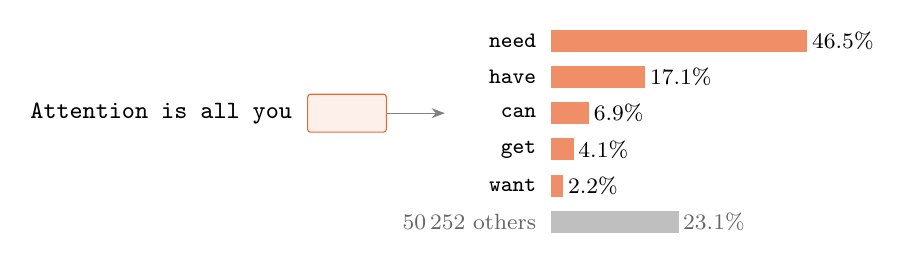
\begin{tikzpicture}[x=1mm, y=1mm, >=Stealth, font=\footnotesize]
  \node[anchor=east, font=\ttfamily\small, inner sep=1pt] (prompt) at (0,0) {Attention is all you};
  \node[draw=ctrl, fill=ctrl!10, rounded corners=1pt, minimum width=10mm, minimum height=4.8mm, anchor=west] (gap) at (1.5,0) {};
  \draw[->, black!50] (gap.east) -- (19,0);
  \foreach \tok/\p [count=\k from 0] in {need/46.5, have/17.1, can/6.9, get/4.1, want/2.2} {
    \node[anchor=east, font=\ttfamily\footnotesize, inner sep=1pt] at (31,{9.2-4.6*\k}) {\tok};
    \fill[ctrl!75] (32.5,{9.2-4.6*\k-1.4}) rectangle ++({0.7*\p},2.8);
    \node[anchor=west, inner sep=1.5pt] at ({32.5+0.7*\p},{9.2-4.6*\k}) {$\p\%$};
  }
  \node[anchor=east, inner sep=1pt, text=black!60] at (31,-13.8) {$50\,252$ others};
  \fill[black!25] (32.5,-15.2) rectangle ++({0.7*23.1},2.8);
  \node[anchor=west, inner sep=1.5pt, text=black!60] at ({32.5+0.7*23.1},-13.8) {$23.1\%$};
\end{tikzpicture}

\medskip
\raggedright
To write, \alert{sample} $i_{t+1}$, append it, and repeat.\footnotemark
\footnotetext{The numbers are those of GPT-2 \citep{radford2019}, the model that this lecture takes apart.}
\end{frame}


% =========================================================================
\begin{frame}{One model, five steps}
\small
Training a language model means computing, approximately,
\[
\hat w\;\approx\;\argmin_{w}\ -\frac1N\sum_{t=1}^{N}\log p_w\big(i_{t+1}\mid i_1,\dots,i_t\big).
\]

\begin{center}
\resizebox{\linewidth}{!}{\gptdiagram{0}}
\end{center}

\smallskip
{\footnotesize Each step with the lines of code that implement it, in the manner of \emph{The Annotated Transformer} \citep{rush2018,huang2022}.\par}
\end{frame}


% =========================================================================
\begin{frame}{Outline}
\tableofcontents
\end{frame}


% #########################################################################
% PART 1: TOKENS
% #########################################################################

% Part 1: tokens.  Figures and numbers: figures/part1_tokenizer.py and figures/part1_embeddings.py.

% =========================================================================
\section{Tokens}

% The frame "Transformers: text for a language model" of lecture 04, without the positions, which
% come back in part 2.  The entries of e_{i_t} are learned: drawn here as random numbers in
% [-1, 1], from a fixed seed.  The indices are those of the tokenizer of GPT-2 (figures/gpt2.py).
\begin{frame}{From text to vectors}
\begin{columns}[c]
\begin{column}{0.57\textwidth}
\centering
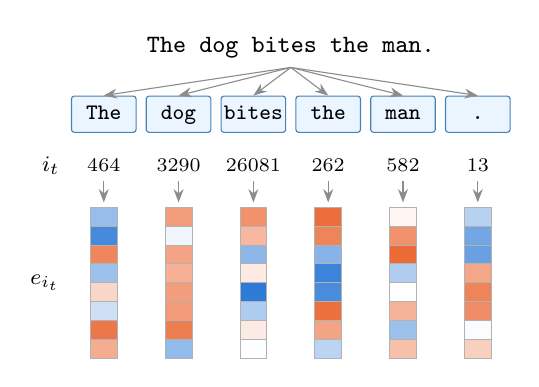
\begin{tikzpicture}[x=0.95cm, y=1cm, >=Stealth, font=\footnotesize,
    tok/.style={draw=boxframe, fill=boxbg, rounded corners=1pt, minimum height=4.6mm, minimum width=8.2mm,
                inner sep=1pt, font=\ttfamily\footnotesize},
    cell/.style={minimum width=3.4mm, minimum height=2.4mm, inner sep=0pt, line width=0.3pt},
    lab/.style={anchor=east, inner sep=1pt}]
  \node[font=\ttfamily\small] (text) at (2.5,0) {The dog bites the man.};
  \pgfmathsetseed{2026}
  \foreach \t/\w/\i in {0/The/464, 1/dog/3290, 2/bites/26081, 3/the/262, 4/man/582, 5/./13} {
    \node[tok] (t\t) at (\t,-0.85) {\strut\w};
    \draw[->, black!45] (text.south) -- (t\t.north);
    \node[font=\scriptsize] (i\t) at (\t,-1.5) {\i};
    \draw[->, black!45] (i\t.south) -- (\t,-1.97);
    \foreach \k in {0,...,7} {
      % e_{i_t}: a random entry in [-1, 1]
      \pgfmathsetmacro\v{rand}
      \pgfmathtruncatemacro\pct{round(100*abs(\v))}
      \pgfmathtruncatemacro\isneg{\v<0}
      \ifnum\isneg=1 \def\pc{posneg}\else\def\pc{ctrl}\fi
      \node[cell, draw=black!30, fill=\pc!\pct!white] at (\t,-2.15-0.24*\k) {};
    }
  }
  \node[lab] at (-0.55,-1.5) {$i_t$};
  \node[lab] at (-0.55,-2.99) {$e_{i_t}$};
\end{tikzpicture}
\end{column}
\begin{column}{0.41\textwidth}
\small
\begin{align*}
i_t&\in\Vocab\\
x_t&=e_{i_t}\in\R^d
\end{align*}

\scriptsize
One learned vector $e_i$ per token of the vocabulary. Drawn: $d=8$.

\medskip
GPT-2: $|\Vocab|=50\,257$ and $d=768$, that is $38.6$ million parameters.
\end{column}
\end{columns}
\end{frame}


% =========================================================================
% Byte-pair encoding, learned on Shakespeare (notebooks/data/tinyshakespeare.txt, 1 115 394
% characters, ASCII).  figures/part1_tokenizer.py runs this listing verbatim (only the path of
% the file differs; the imports, re and collections.Counter, are not shown) and prints the
% output below.  The table comes from the same script: a faster version of the same algorithm,
% which agrees with the listing on the first 100 merges, run until every word is one symbol
% (21 279 merges).  "gentleman" occurs 77 times in the text, "Erlangen" never.  Tokens per
% character: the length of the text in symbols after k merges over its 1 115 394 characters
% (0.613, 0.388, 0.277; after all 21 279 merges 0.264, and Erlangen is Er|l|ang|en).  The
% output is printed on one line; it is broken in two here.  The same numbers as a curve, with
% the declaration in English and German and GPT-2: images/bpe_compression.pdf (not used here).
\begin{frame}[fragile]{Byte-pair encoding: merge the most frequent pair}
\def\tokbar{\textcolor{black!40}{|}}
\begin{lstlisting}
text = open("tinyshakespeare.txt", encoding="latin-1").read()  # 1115394 bytes
words = Counter(re.findall(r" ?\w+| ?[^\w\s]+|\s+", text))  # ' the': 5370
vocab = {chr(i): bytes([i]) for i in range(256)}           # 256 bytes
for new in map(chr, range(256, 268)):                      # 12 new symbols
    pairs = Counter()
    for w, n in words.items():
        for a, b in zip(w, w[1:]): pairs[a + b] += n       # neighbouring pairs
    ab, count = pairs.most_common(1)[0]                    # the most frequent
    vocab[new] = vocab[ab[0]] + vocab[ab[1]]
    words = {w.replace(ab, new): n for w, n in words.items()}  # merge it
    print(vocab[new], count, end="  ")
\end{lstlisting}
\begin{lstlisting}[style=output]
> b' t' 23835  b'he' 18203  b' a' 13541  b'ou' 12730  b' s' 12287  b' m' 10783
  b'in' 10606  b' w' 10546  b're' 9843  b'ha' 9673  b'nd' 8730  b' the' 8683
\end{lstlisting}
\scriptsize
\setlength{\tabcolsep}{4pt}
\begin{tabularx}{\textwidth}{@{}r X X r@{}}
\toprule
merges\footnotemark & \texttt{\textvisiblespace gentleman} (77 times) & \texttt{\textvisiblespace Erlangen} (never) & tokens per character \\
\midrule
0 & \texttt{\textvisiblespace\tokbar g\tokbar e\tokbar n\tokbar t\tokbar l\tokbar e\tokbar m\tokbar a\tokbar n}
  & \texttt{\textvisiblespace\tokbar E\tokbar r\tokbar l\tokbar a\tokbar n\tokbar g\tokbar e\tokbar n} & 1.00 \\
100 & \texttt{\textvisiblespace g\tokbar ent\tokbar le\tokbar m\tokbar an}
  & \texttt{\textvisiblespace\tokbar E\tokbar r\tokbar l\tokbar an\tokbar g\tokbar en} & 0.61 \\
1000 & \texttt{\textvisiblespace gentle\tokbar man}
  & \texttt{\textvisiblespace E\tokbar r\tokbar l\tokbar an\tokbar g\tokbar en} & 0.39 \\
10\,000 & \texttt{\textvisiblespace gentleman}
  & \texttt{\textvisiblespace E\tokbar r\tokbar l\tokbar ang\tokbar en} & 0.28 \\
\bottomrule
\end{tabularx}
\footnotetext{Byte-pair encoding: for compression \citep{gage1994}, for words \citep{sennrich2016}, on bytes \citep{radford2019}.}
\end{frame}


% =========================================================================
% The tokenizer of GPT-2 (Radford et al., 2019): 256 bytes + 50 000 merges + <|endoftext|>.
% figures/part1_tokenizer.py prints every example (gpt2.encode, exact GPT-2 tokenization) and
% draws tokens_udhr.pdf: article 1 of the Universal Declaration of Human Rights (OHCHR, English
% and German, via the "UDHR in Unicode" project), one box per token, the space of a word
% inside its first token.  Tokens per word over the 30 articles (parallel, 50 paragraphs):
% English 1 361 words, 1 570 tokens; German 1 278 words, 3 598 tokens.  Vocabulary sizes:
% cl100k_base (GPT-4) 100 256 merged tokens + 5 special ones, o200k_base (GPT-4o and later)
% 199 998 + 2 special ones = 200 000, counted in OpenAI's files (the largest ids are 100 276 and
% 200 018, so tiktoken's n_vocab is 100 277 and 200 019); Llama 3 "128K" (128 000 + 256 special tokens
% in Meta's tokenizer.py).  Not on the slide: Qwen3, 151 669 (Yang et al., 2025).
% GPT-2: 256 bytes + 50 000 merges + <|endoftext|>, checked against encoder.json and vocab.bpe.
\begin{frame}{The tokens of GPT-2 are neither words nor letters}
\def\tokbar{\textcolor{black!40}{|}}
\centering
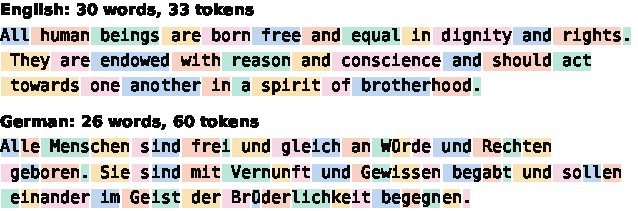
\includegraphics{tokens_udhr.pdf}

\medskip
\scriptsize
\renewcommand{\arraystretch}{1.1}
\begin{tabularx}{\textwidth}{@{}l X@{}}
\toprule
letters & \texttt{strawberry} $\to$ \texttt{st\tokbar raw\tokbar berry};\quad \texttt{\textvisiblespace strawberry} $\to$ one token: how many r? \\
spaces, capitals & \texttt{the} 1169,\; \texttt{\textvisiblespace the} 262,\; \texttt{The} 464,\; \texttt{\textvisiblespace The} 383: four unrelated tokens \\
numbers & \texttt{\textvisiblespace 2026} $\to$ \texttt{\textvisiblespace 20\tokbar 26};\quad \texttt{\textvisiblespace 1234567} $\to$ \texttt{\textvisiblespace 123\tokbar 45\tokbar 67} \\
German & \texttt{\textvisiblespace Prüfungsordnung} $\to$ \texttt{\textvisiblespace Pr\tokbar ü\tokbar f\tokbar ung\tokbar s\tokbar ord\tokbar n\tokbar ung} \\
bytes & \texttt{Übung} $\to$ \texttt{\textbackslash xc3\tokbar\textbackslash x9c\tokbar b\tokbar ung}: the two bytes of Ü, cut apart \\
vocabulary & GPT-2 $50\,257=256+50\,000+1$;\quad GPT-4o $200\,000$;\quad Llama 3 128K\footnotemark \\
\bottomrule
\end{tabularx}

\medskip
\raggedright
All 30 articles: \alert{1.15} tokens per English word, \alert{2.82} per German word.
\footnotetext{\citet{radford2019}; \texttt{o200k\_base} of tiktoken \citep{tiktoken2022}; \citet{grattafiori2024}.}
\end{frame}


% =========================================================================
% Numbers:
% figures/part1_embeddings.py.  Nearest rows of the token embedding in cosine similarity,
% nothing filtered; \textvisiblespace is the space that starts a GPT-2 token.
\begin{frame}{Similar tokens, similar vectors}
\small
The vectors $e_i$ are learned with everything else. In GPT-2, after training:

\medskip
\scriptsize
\renewcommand{\arraystretch}{1.25}
\setlength{\tabcolsep}{3pt}
\begin{tabular*}{\textwidth}{@{}l@{\extracolsep{\fill}}llll@{}}
\toprule
token $i$ & \multicolumn{4}{l}{nearest tokens $j$, by $\cos(e_i,e_j)$} \\
\midrule
\texttt{\textvisiblespace Germany}     & \texttt{Germany} .86      & \texttt{\textvisiblespace German} .75     & \texttt{German} .71        & \texttt{\textvisiblespace France} .70 \\
\texttt{\textvisiblespace mathematics} & \texttt{\textvisiblespace Mathematics} .82 & \texttt{\textvisiblespace mathematical} .78 & \texttt{\textvisiblespace maths} .76 & \texttt{\textvisiblespace math} .75 \\
\texttt{\textvisiblespace theorem}     & \texttt{\textvisiblespace hypothesis} .54 & \texttt{\textvisiblespace fallacy} .52 & \texttt{\textvisiblespace mathematic} .52 & \texttt{\textvisiblespace mathematician} .52 \\
\texttt{\textvisiblespace Monday}      & \texttt{\textvisiblespace Tuesday} .89  & \texttt{\textvisiblespace Thursday} .85   & \texttt{\textvisiblespace Wednesday} .84 & \texttt{\textvisiblespace Friday} .82 \\
\texttt{\textvisiblespace seven}       & \texttt{\textvisiblespace six} .87      & \texttt{\textvisiblespace eight} .86      & \texttt{\textvisiblespace five} .85      & \texttt{\textvisiblespace nine} .85 \\
\texttt{\textvisiblespace river}       & \texttt{\textvisiblespace rivers} .78   & \texttt{\textvisiblespace River} .74      & \texttt{\textvisiblespace lake} .66      & \texttt{\textvisiblespace creek} .64 \\
\bottomrule
\end{tabular*}

\medskip
\small
Two random tokens: $\cos(e_i,e_j)=0.27$ on average. \alert{Nobody told the model} that Monday and Tuesday belong together.
\end{frame}


% #########################################################################
% PART 2: ATTENTION
% #########################################################################

% Part 2: attention.  Figures and numbers: figures/part0_recurrent.py, figures/part2_attention.py
% and figures/part2_gpt2_attention.py.

% =========================================================================
\section{Attention}

% =========================================================================
% The sample is Shannon's "second-order word approximation" (1948, section 3), verbatim: each word
% is drawn given the one before it, with the frequencies of English text.
\begin{frame}{Language models before attention}
\small
\begin{mathbox}{C.~Shannon, 1948 \citep{shannon1948}: each word drawn given the one before, from counts}
\ttfamily\footnotesize THE HEAD AND IN FRONTAL ATTACK ON AN ENGLISH WRITER THAT THE CHARACTER OF THIS POINT IS THEREFORE ANOTHER METHOD FOR THE LETTERS THAT THE TIME OF WHO EVER TOLD THE PROBLEM FOR AN UNEXPECTED
\end{mathbox}

\bigskip
\centering
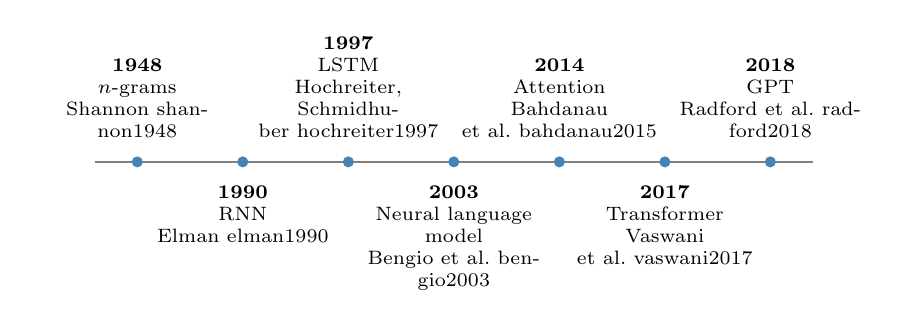
\begin{tikzpicture}[x=1.34cm, y=1cm, every node/.style={font=\scriptsize}]
  \draw[gray, line width=0.8pt] (-0.4,0) -- (6.4,0);
  \foreach \x/\yr/\txt/\anc/\dy in {
     0/1948/{\alert{$n$-grams}\\Shannon~\citep{shannon1948}}/south/0.18,
     1/1990/{\alert{RNN}\\Elman~\citep{elman1990}}/north/-0.18,
     2/1997/{\alert{LSTM}\\Hochreiter, Schmidhuber~\citep{hochreiter1997}}/south/0.18,
     3/2003/{\alert{Neural language}\\\alert{model}\\Bengio et~al.~\citep{bengio2003}}/north/-0.18,
     4/2014/{\alert{Attention}\\Bahdanau et~al.~\citep{bahdanau2015}}/south/0.18,
     5/2017/{\alert{Transformer}\\Vaswani et~al.~\citep{vaswani2017}}/north/-0.18,
     6/2018/{\alert{GPT}\\Radford et~al.~\citep{radford2018}}/south/0.18}
  {
    \fill[boxframe] (\x,0) circle (2pt);
    \node[anchor=\anc, align=center, text width=2.55cm] at (\x,\dy) {\textbf{\yr}\\\txt};
  }
\end{tikzpicture}

\bigskip
\raggedright
From 1990 to 2017 the model of a sequence is \alert{recurrent}: it reads one token at a time.
\end{frame}


% =========================================================================
% Opening.  Figure: figures/part0_recurrent.py (recurrent_panels.pdf); three layers of width 64
% with PyTorch's default initialization: nn.RNN (tanh), nn.LSTM, nn.MultiheadAttention (4 heads).
% Left: |d y_n / d x_t| (operator norm) at initialization, n = 100, geometric mean over 20 seeds:
% per step the RNN loses a factor 0.466, the LSTM 0.617; one attention layer stays between
% 1.3e-2 and 2.0e-2 at every distance n - t >= 1.  Right: "recall the first token" (one of 8
% symbols, then n - 1 fillers from 8 other symbols; chance 12.5%), one budget for all (Adam 3e-3,
% batches of 64, at most 2000 steps), accuracy on 4096 test sequences, mean of 3 seeds, for
% n = 5, 10, 20, 50, 100, 200: RNN 100, 100, 74.8, 10.9, 12.8, 13.5%; LSTM 100, 100, 41.7, 12.5,
% 12.6, 12.5%; attention 100% for every n, within 100 steps.  At n = 20 the RNN learns the task
% for 2 seeds of 3, the LSTM for 1 of 3.  An LSTM with its forget gates opened (bias + 1, seed 0)
% learns n = 20 but not n = 50 or 100.
\begin{frame}{Recurrent networks read one token at a time}
\small
\tikzset{
  tok/.style={circle, draw=boxframe, fill=boxbg, inner sep=0pt, minimum size=2.6mm},
  edge/.style={black!35, line width=0.4pt},
  hot/.style={ctrl, line width=0.9pt},
}
\begin{columns}[T]
\begin{column}{0.5\textwidth}
\centering
\alert{Recurrent}: $h_t=\sigma(Wh_{t-1}+Ux_t)$\\[1pt]
\begin{tikzpicture}[x=7.5mm, y=1mm, >=Stealth, font=\scriptsize]
  \foreach \i in {1,...,6} \node[tok] (r\i) at (\i,0) {};
  \foreach \i [evaluate=\i as \j using int(\i+1)] in {1,...,5} \draw[->, hot] (r\i) -- (r\j);
  \node[below=0.5mm] at (r1.south) {$x_1$};
  \node[below=0.5mm] at (r6.south) {$x_n$};
  \node[above, text=ctrl, inner sep=1pt] at (3.5,1.6) {$n-1$ steps from $x_1$ to $x_n$};
\end{tikzpicture}
\end{column}
\begin{column}{0.5\textwidth}
\centering
\alert{Self-attention}: $x_t\leftarrow x_t+\sum_s a_{ts}(x)\,Vx_s$\\[1pt]
\begin{tikzpicture}[x=7.5mm, y=1mm, >=Stealth, font=\scriptsize]
  \foreach \i in {1,...,6} \node[tok] (a\i) at (\i,0) {};
  % every pair (t, s) is one edge; the arc rises with the distance s - t
  \foreach \i in {1,...,5} \foreach \j in {\i,...,6}
    {\ifnum\i<\j \draw[edge] (a\i.north) .. controls +({0.12*(\j-\i)},{1.2*(\j-\i)}) and +({-0.12*(\j-\i)},{1.2*(\j-\i)}) .. (a\j.north);\fi}
  \draw[hot] (a1.north) .. controls +(0.6,6) and +(-0.6,6) .. (a6.north);
  \node[below=0.5mm] at (a1.south) {$x_1$};
  \node[below=0.5mm] at (a6.south) {$x_n$};
  \node[above, text=ctrl, inner sep=1pt] at (3.5,5.8) {$1$ step from $x_1$ to $x_n$};
\end{tikzpicture}
\end{column}
\end{columns}

\smallskip
{\footnotesize \alert{LSTM} \citep{hochreiter1997}: $c_t=f_t\odot c_{t-1}+i_t\odot g_t$, gates $f_t,i_t\in(0,1)^d$. Along $c$ the gradient is multiplied by $f_t$, not by $W^\top\sigma'$ \citep{bengio1994}.\par}

\centering
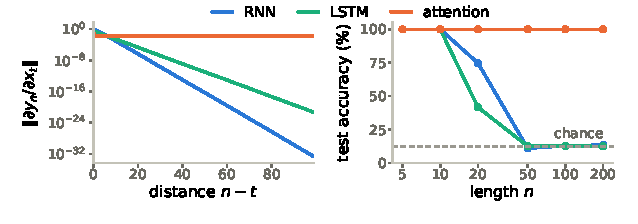
\includegraphics{recurrent_panels.pdf}
\end{frame}


% =========================================================================
% Table 1 of Vaswani et al. (2017) (arXiv:1706.03762, p. 6), recurrent and self-attention rows
% only (n: length, d: width).  Timings: figures/part0_recurrent.py, part (c): one forward pass of
% nn.RNN(64, 64) and nn.MultiheadAttention(64, 4) on one sequence, the minimum over repetitions,
% two runs on an idle 16-core machine.  nn.RNN at n = 1024: 7.2 and 7.1 ms with one thread, 7.3
% and 7.2 ms with four (7 us per token, no faster with more threads).  Attention at n = 1024: 8.8
% and 8.8 ms with one thread, 2.6 and 2.6 ms with four.  At n = 4096 attention is slower than the
% RNN on this CPU (138 and 141 ms against 31 and 30 ms, one thread): it does n/d = 64 times more
% operations.
\begin{frame}{Recurrence against attention, per layer}
\small
\centering
\renewcommand{\arraystretch}{1.1}
\begin{tabular}{@{}l c c c@{}}
\toprule
 & \textbf{Operations} & \textbf{Sequential steps} & \textbf{Longest path} \\
\midrule
Recurrent & $O(n\,d^2)$ & $O(n)$ & $O(n)$ \\
Self-attention & $O(n^2d)$ & \alert{$O(1)$} & \alert{$O(1)$} \\
\bottomrule
\end{tabular}

\smallskip
{\footnotesize Table~1 of \citet{vaswani2017}; $n$ tokens of width $d$.\par}

\medskip
\raggedright
Measured on a CPU, one sequence of $n=1024$ tokens, $d=64$: \texttt{nn.RNN} takes $7$\,ms with 1 thread and $7$\,ms with 4, one token after the other. Attention: $9$\,ms with 1 thread, $2.6$\,ms with 4.

\medskip
\alert{Attention does more operations, but all at once, and any two tokens are one step apart.}
\end{frame}


% =========================================================================
% Figure and listing: figures/part2_attention.py, section 1 (the listing runs inside the script,
% which prints its output).  The figure: a query at 50 degrees and eight keys at 0, 45, ..., 315
% degrees on the unit circle; the largest weight, on k_2, is 0.27, 0.59 and 0.97 for beta = 1, 4, 16.
\begin{frame}[fragile,t]{Attention is a differentiable look-up table}
\small
Keys $k_s$, values $v_s$, a query $q$.
\[
\text{\alert{Look-up:}}\ \ \text{out}=v_{s^\ast},\ \ k_{s^\ast}=q.
\qquad
\text{\alert{Attention:}}\ \ \text{out}=\sum_s\softmax_s\big(\ctrl{\beta}\,\langle q,k_s\rangle\big)\,v_s .
\]
\begin{onlyenv}<1>
\medskip
\centering
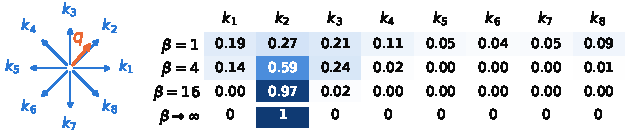
\includegraphics{lookup_weights.pdf}

\medskip
\raggedright
The weights $\softmax_s(\ctrl{\beta}\langle q,k_s\rangle)$ for one query and eight keys on the unit circle.

\medskip
\alert{$\beta\to\infty$:} the value of the nearest key, a look-up.\footnotemark
\end{onlyenv}
\begin{onlyenv}<2>
\begin{lstlisting}[belowskip=2pt]
table = {"a": 1.0, "b": 2.0, "c": 3.0}
table["b"]                                         # look-up: an exact match
keys = torch.tensor([[1.0, 0.0], [0.6, 0.8], [0.0, 1.0]])     # a, b, c
values = torch.tensor([1.0, 2.0, 3.0])
q = torch.tensor([0.6, 0.8], requires_grad=True)   # the query: key b
w = (16 * keys @ q).softmax(0); out = w @ values   # attention, beta = 16
out.backward(); w.data, out.data, q.grad
\end{lstlisting}
\begin{lstlisting}[style=output]
> 2.0
> tensor([0.0016, 0.9593, 0.0391]) tensor(2.0375) tensor([-0.3719,  0.1416])
\end{lstlisting}

\smallskip
\alert{Finite $\beta$:} the output has a gradient in $q$, $k_s$ and $v_s$. \alert{The table can be learned.}
\end{onlyenv}
\footnotetext<1>{With a kernel for the softmax: the regression of Nadaraya and Watson, 1964 \citep{nadaraya1964,watson1964}.}
\end{frame}


% =========================================================================
% The table of L. Weng's post "Attention? Attention!" (2018), in the notation of this lecture:
% her s_t (the state of the decoder) is the query q, her h_i (a state of the encoder) the key k, and
% her n, "the dimension of the source hidden state", is d.  Checked against the papers: Graves et al.
% (2014, eq. 5-6) compare a key with the rows of a memory and multiply the cosine by a key strength;
% Bahdanau et al. (2015, appendix A.1.2); Luong et al. (2015, section 3.1); Vaswani et al. divide by
% the square root of the dimension d_k of the queries and keys.
\begin{frame}{Attention before 2017: a table of scores}
\small
\alert{2014.} A recurrent translator squeezes the sentence into one vector. Bahdanau et~al.: let each new word look back at all the states $h_1,\dots,h_n$ of the input,
\[
c_t=\sum_{s=1}^n a_{ts}\,h_s,\qquad a_{ts}=\softmax_s\big(\score(q_t,h_s)\big).
\]

\footnotesize
{\centering
\renewcommand{\arraystretch}{1.15}
\begin{tabular}{@{}l l l@{}}
\toprule
\textbf{Name} & \textbf{$\score(q,k)$} & \textbf{Table of L.~Weng \citep{weng2018}} \\
\midrule
content-based & $\cos(q,k)$ & Graves et~al., 2014 \citep{graves2014} \\
additive & $v^\top\tanh\big(W[q;k]\big)$ & Bahdanau et~al., 2015 \citep{bahdanau2015} \\
location-based & $Wq$\quad (no key) & Luong et~al., 2015 \citep{luong2015} \\
general & $q^\top Wk$ & Luong et~al., 2015 \citep{luong2015} \\
dot product & $q^\top k$ & Luong et~al., 2015 \citep{luong2015} \\
\rowcolor{ctrl!12}\alert{scaled dot product} & $q^\top k/\sqrt d$ & Vaswani et~al., 2017 \citep{vaswani2017} \\
\bottomrule
\end{tabular}\par}

\smallskip
\small
\alert{2017.} The score is not new: $\langle Qx_t,Kx_s\rangle=x_t^\top(Q^\top K)\,x_s$ is the general one. New is what was removed, the recurrent network: \emph{Attention is all you need}.
\end{frame}


% =========================================================================
% The figure: figures/part2_gpt2_attention.py (gpt2_attention_one.pdf).  The sentence is the example
% of Wang et al. (2023), with <|endoftext|> first (the token GPT-2 saw between documents); head 9.9
% is head 9 of block 9, both counted from 0.  Without <|endoftext|>: 0.36 on Mary, 0.36 on "When";
% next token Mary 0.45, John 0.06.
\begin{frame}[fragile]{Self-attention}
\small
Queries, keys, values: all from the same tokens, $q_t=Qx_t$, $k_s=Kx_s$, $v_s=Vx_s$.
\[
\ctrl{a_{ts}}=\softmax_s\Big(\frac{\langle Qx_t,Kx_s\rangle}{\sqrt d}\Big),\qquad\quad
x_t\;\leftarrow\;x_t+\sum_{s=1}^n\ctrl{a_{ts}}\,Vx_s .
\]
\begin{lstlisting}
def attention(q, k, v):                      # rows: one per token
    scores = q @ k.T / k.shape[-1] ** 0.5    # (n, n): every pair of tokens
    a = scores.softmax(-1)                   # each row sums to 1
    return a @ v                             # weighted means of the values
\end{lstlisting}

\centering
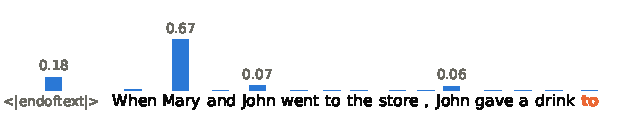
\includegraphics{gpt2_attention_one.pdf}

\raggedright\footnotesize
GPT-2, one head \citep{wang2023}: the weights $\ctrl{a_{ns}}$ of the last token. Next token: \texttt{Mary} $0.68$, \texttt{John} $0.02$.
\end{frame}


% =========================================================================
% Figure and numbers: figures/part2_attention.py, section 2.  n = 64 queries and keys with
% independent N(0, 1) entries, 200 draws for each d (the set-up of notebooks/15_transformers.ipynb,
% section 2).  Left: the largest weight of a row, mean over 12 800 rows: 0.947 without the factor
% at d = 1024, 0.107 with it (1/n = 0.016).  Right: the median Frobenius norm of the Jacobian of the
% softmax: 2.8e-4 without, 0.18 with the factor at d = 1024; 55% of the rows are below 1e-3
% without it, none with it.  The empirical Var <q,k> is 1022.9 at d = 1024.
\begin{frame}{Why the $1/\sqrt d$}
\small
If $q,k\in\R^d$ have independent entries of mean $0$ and variance $1$,
\[
\E\langle q,k\rangle=\sum_{j=1}^d\E q_j\,\E k_j=0,\qquad
\Var\langle q,k\rangle=\sum_{j=1}^d\E q_j^2\,\E k_j^2=d.
\]
Scores $z$ of size $\sqrt d$ saturate $a=\softmax(z)$, and its Jacobian
$\partial a/\partial z=\operatorname{diag}(a)-aa^\top$ vanishes: \alert{no gradient reaches $Q$ and $K$}.

\centering
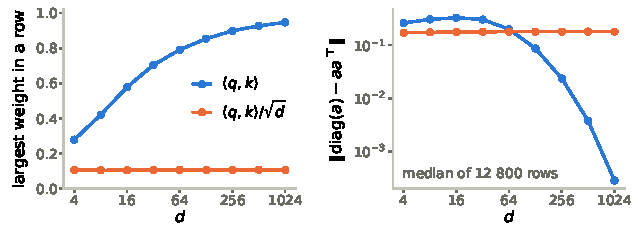
\includegraphics{scaling_softmax.pdf}

{\raggedright\footnotesize $n=64$ tokens, $q_t$ and $k_s$ drawn $200$ times for each $d$.\par}
\end{frame}


% =========================================================================
% Figure and numbers: figures/part2_gpt2_attention.py (gpt2_attention_heads.pdf).  The four
% heads were picked by looking at all 144 on this sentence; the script ranks them.
\begin{frame}{Multi-head attention}
\small
$H$ heads, each with its own $Q_h,K_h,V_h\in\R^{(d/H)\times d}$ and $O_h\in\R^{d\times(d/H)}$:
\[
x_t\leftarrow x_t+\sum_{h=1}^{H}O_h\sum_s a^h_{ts}(x)\,V_hx_s,\qquad
a^h_{ts}(x)=\softmax_s\Big(\frac{\langle Q_hx_t,K_hx_s\rangle}{\sqrt{d/H}}\Big).
\]
GPT-2 small: $d=768$, $H=12$ heads of width $64$ in each of $12$ blocks.

\medskip
\centering
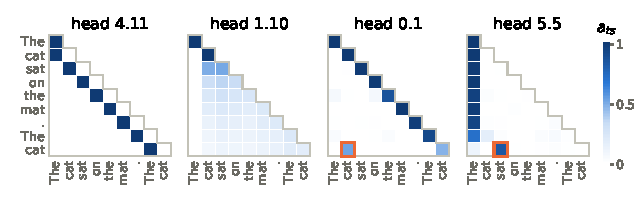
\includegraphics{gpt2_attention_heads.pdf}

\raggedright\footnotesize
Four of its 144 heads: the previous token; the tokens so far, alike; the same token; the token after the earlier \texttt{cat} ($0.84$).
\end{frame}


% =========================================================================
% The four panels: figures/part2_attention.py, section 3.  Six tokens in R^8 (one per row, blue
% negative, orange positive), f(x) = x + attention(x) for nn.MultiheadAttention(8, 2) with PyTorch's
% default initialization (seed 0), the permutation pi = (1, 4, 2, 6, 3, 5): row t of Px is token pi(t).
% The numbers beside the rows are the token indices.  Printed by the script:
% max |f(Px) - Pf(x)| = 1.2e-7 (float32); with the causal mask 0.244 (the update f(x) - x is at
% most 0.283); with sinusoidal positions p_t added, the update attention(x + p) differs by 0.137
% (it is at most 0.402).  The positions are compared on the update only: f(x + p) contains x + p,
% and p - Pp alone would break the identity.  The listing of the second step is the one of lecture 03
% (frame "Six layers, and what they assume") with the mask added; the script runs it.
\tikzset{
  cdsquare/.style={x=1mm, y=1mm, >=Stealth, font=\footnotesize},
  cdcorner/.style={inner sep=0pt},
  cdlabel/.style={font=\footnotesize, inner sep=1.5pt, text height=1.7ex, text depth=0.5ex},
}
\begin{frame}[fragile]{Self-attention is permutation equivariant}
\begin{mathbox}{Proposition}
Let $f(x)_t=x_t+\sum_s a_{ts}(x)\,Vx_s$ and $(Px)_t=x_{\pi(t)}$ for a permutation $\pi$ of $\{1,\dots,n\}$. Then $f(Px)=P\,f(x)$.
\end{mathbox}

\smallskip
\begin{onlyenv}<1>
\begin{columns}[c]
\begin{column}{0.47\textwidth}
\centering
\begin{tikzpicture}[cdsquare]
  \node[cdcorner] (x)   at (0,0)    {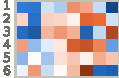
\includegraphics{equivariance_x.pdf}};
  \node[cdcorner] (fx)  at (29,0)   {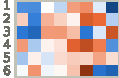
\includegraphics{equivariance_fx.pdf}};
  \node[cdcorner] (Px)  at (0,-25)  {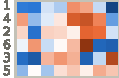
\includegraphics{equivariance_Px.pdf}};
  \node[cdcorner] (fPx) at (29,-25) {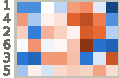
\includegraphics{equivariance_fPx.pdf}};
  \draw[->] ([xshift=1mm]x.east)  -- node[above] {$f$} ([xshift=-1mm]fx.west);
  \draw[->] ([xshift=1mm]Px.east) -- node[below] {$f$} ([xshift=-1mm]fPx.west);
  \draw[->] ([yshift=-1mm]x.south)  -- node[left]  {$P$} ([yshift=1mm]Px.north);
  \draw[->] ([yshift=-1mm]fx.south) -- node[right] {$P$} ([yshift=1mm]fPx.north);
  \node[cdlabel, above] at (x.north)   {$x$};
  \node[cdlabel, above] at (fx.north)  {$f(x)$};
  \node[cdlabel, below] at (Px.south)  {$Px$};
  \node[cdlabel, below] at (fPx.south) {$f(Px)=P\,f(x)$};
\end{tikzpicture}
\end{column}
\begin{column}{0.51\textwidth}
\footnotesize
\emph{Proof idea.} $a_{ts}(x)$ depends on the pair $(x_t,x_s)$ and on a sum over all tokens, so $a_{ts}(Px)=a_{\pi(t)\pi(s)}(x)$. A sum over $s$ does not see the order:
\[
\begin{aligned}
f(Px)_t&=x_{\pi(t)}+\textstyle\sum_s a_{\pi(t)\pi(s)}(x)\,Vx_{\pi(s)}\\
&=f(x)_{\pi(t)}.
\end{aligned}
\]
Measured on the six tokens drawn: $\max|f(Px)-Pf(x)|=1.2\cdot10^{-7}$.
\end{column}
\end{columns}
\end{onlyenv}
\begin{onlyenv}<2>
\small
The check of lecture 03, and what breaks it:
\begin{lstlisting}[belowskip=2pt]
x = torch.randn(10, 32)                    # 10 tokens in R^32
attn = nn.MultiheadAttention(32, 4)        # 4 heads
f = lambda x, mask=None: x + attn(x, x, x, attn_mask=mask)[0]
p = torch.randperm(10)                     # a permutation
torch.allclose(f(x[p]), f(x)[p], atol=1e-6)
\end{lstlisting}
\begin{lstlisting}[style=output]
> True
\end{lstlisting}
\begin{lstlisting}[belowskip=2pt]
mask = torch.ones(10, 10).triu(1).bool()   # no looking ahead
torch.allclose(f(x[p], mask), f(x, mask)[p], atol=1e-6)
\end{lstlisting}
\begin{lstlisting}[style=output]
> False
\end{lstlisting}

\smallskip
\alert{Order enters only through the mask and the positions}: the next two slides.
\end{onlyenv}
\end{frame}


% =========================================================================
% The frame "Transformers: text for a language model" of lecture 04.  The values of p_t (d = 8,
% t = 0..5) are computed below with the formula on the right.  The entries of e_{i_t} are the
% random numbers of the frame "Tokens become vectors" (the same seed).
\begin{frame}{Positional encoding}
\begin{columns}[c]
\begin{column}{0.57\textwidth}
\centering
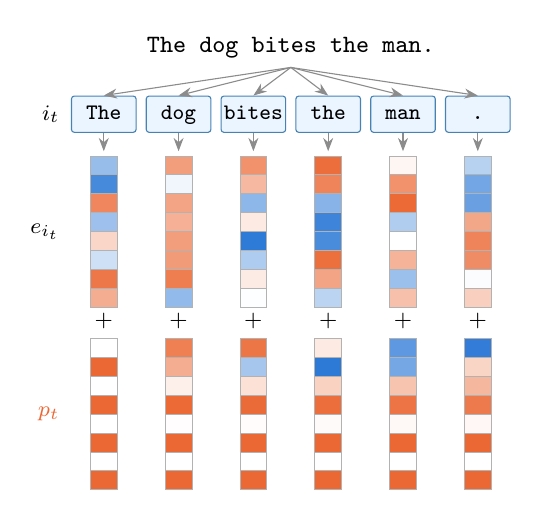
\begin{tikzpicture}[x=0.95cm, y=1cm, >=Stealth, font=\footnotesize,
    tok/.style={draw=boxframe, fill=boxbg, rounded corners=1pt, minimum height=4.6mm, minimum width=8.2mm,
                inner sep=1pt, font=\ttfamily\footnotesize},
    cell/.style={minimum width=3.4mm, minimum height=2.4mm, inner sep=0pt, line width=0.3pt},
    lab/.style={anchor=east, inner sep=1pt}]
  \node[font=\ttfamily\small] (text) at (2.5,0) {The dog bites the man.};
  \pgfmathsetseed{2026}
  \foreach \t/\w in {0/The, 1/dog, 2/bites, 3/the, 4/man, 5/.} {
    \node[tok] (t\t) at (\t,-0.85) {\strut\w};
    \draw[->, black!45] (text.south) -- (t\t.north);
    \draw[->, black!45] (t\t.south) -- (\t,-1.32);
    \foreach \k in {0,...,7} {
      % e_{i_t}: a random entry in [-1, 1]
      \pgfmathsetmacro\v{rand}
      \pgfmathtruncatemacro\pct{round(100*abs(\v))}
      \pgfmathtruncatemacro\isneg{\v<0}
      \ifnum\isneg=1 \def\pc{posneg}\else\def\pc{ctrl}\fi
      \node[cell, draw=black!30, fill=\pc!\pct!white] at (\t,-1.5-0.24*\k) {};
      % p_t: sin and cos of omega_j t, omega_j = 10000^(-2j/d), in neighbouring coordinates
      \pgfmathsetmacro\angle{10000^(-2*floor(\k/2)/8)*\t}
      \pgfmathsetmacro\v{mod(\k,2)==0 ? sin(\angle r) : cos(\angle r)}
      \pgfmathtruncatemacro\pct{round(100*abs(\v))}
      \pgfmathtruncatemacro\isneg{\v<0}
      \ifnum\isneg=1 \def\pc{posneg}\else\def\pc{ctrl}\fi
      \node[cell, draw=black!30, fill=\pc!\pct!white] at (\t,-3.82-0.24*\k) {};
    }
    \node at (\t,-3.47) {$+$};
  }
  \node[lab] at (-0.55,-0.85) {$i_t$};
  \node[lab] at (-0.55,-2.34) {$e_{i_t}$};
  \node[lab] at (-0.55,-4.66) {$\ctrl{p_t}$};
\end{tikzpicture}
\end{column}
\begin{column}{0.41\textwidth}
\small
\begin{align*}
x_t&=e_{i_t}+\ctrl{p_t}\\
\ctrl{p_t}&=\big(\sin\omega_jt,\ \cos\omega_jt\big)_{j<d/2}\\
\omega_j&=10000^{-2j/d}
\end{align*}

\scriptsize
Without \ctrl{$p_t$}, \texttt{The man bites the dog.} gives the same vectors in another order, and attention does not see the order.
\end{column}
\end{columns}
\end{frame}


% =========================================================================
% Figure, listing and output: figures/part2_attention.py, section 4 (the listing runs inside the
% script with torch.manual_seed(0); the figure shows its tensors).  The six tokens of the running
% sentence are random vectors in R^16 and Q, K, V a random layer: the weights are not those of a
% trained model.
\begin{frame}[fragile,t]{Masking: no looking ahead}
\small
In a language model position $t$ uses the positions $s\le t$ only: the scores above the diagonal are set to $-\infty$ before the softmax.

\medskip
\begin{onlyenv}<1>
\centering
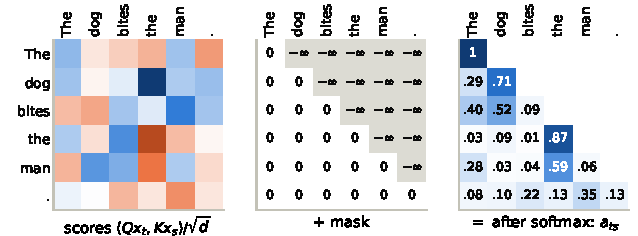
\includegraphics{mask_matrices.pdf}

{\raggedright\footnotesize A random layer: $x_t\in\R^{16}$, $Q,K,V$ with $N(0,1/16)$ entries. Each row of $a$ sums to $1$.\par}
\end{onlyenv}
\begin{onlyenv}<2>
\lstset{aboveskip=0pt, belowskip=0pt}
\begin{lstlisting}
x = torch.randn(6, 16)                    # 6 tokens in R^16
Q, K, V = torch.randn(3, 16, 16) / 4      # one random layer
mask = torch.tril(torch.ones(6, 6)) == 0  # True above the diagonal
def attend(x, mask):
    s = (x @ Q) @ (x @ K).T / 4           # scores / sqrt(d)
    return s.masked_fill(mask, -torch.inf).softmax(-1) @ (x @ V)
y = x.clone(); y[-1] = torch.randn(16)    # change the last token
same = lambda m: torch.allclose(attend(x, m)[:5], attend(y, m)[:5])
print(same(mask), same(mask & False))     # with, without the mask
\end{lstlisting}
\begin{lstlisting}[style=output]
> True False
\end{lstlisting}
\alert{With the mask the outputs at $t<n$ do not see token $n$}; without it they do.
\end{onlyenv}
\end{frame}


% #########################################################################
% PART 3: THE TRANSFORMER
% #########################################################################

% Part 3: the transformer.  The model is figures/gpt2.py; figures and numbers:
% figures/part3_sampling.py and figures/part3_particles.py.

% =========================================================================
\section{The transformer}

\begin{frame}{The transformer block}
\centering
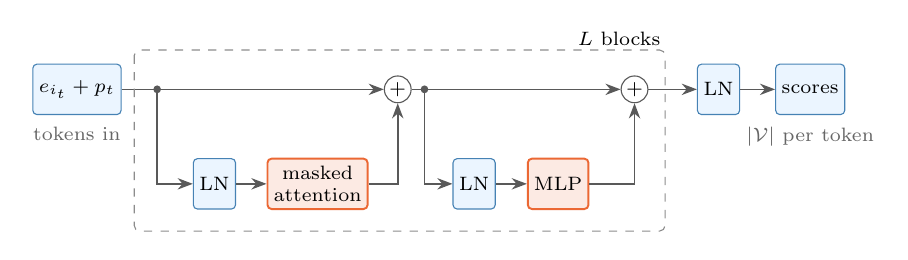
\begin{tikzpicture}[x=0.97mm, y=1mm, >=Stealth, font=\scriptsize,
    op/.style={draw=boxframe, fill=boxbg, rounded corners=1.5pt, minimum height=6.4mm, inner sep=2.2pt, align=center},
    hot/.style={draw=ctrl, fill=ctrl!14, line width=0.7pt},
    plus/.style={circle, draw=black!65, fill=white, inner sep=0pt, minimum size=3.4mm, font=\scriptsize},
    wire/.style={->, black!65, line width=0.55pt}]
  % the residual stream, left to right
  \node[op] (emb) at (7,0) {$e_{i_t}+p_t$};
  \node[plus] (p1) at (49,0) {$+$};
  \node[plus] (p2) at (80,0) {$+$};
  \node[op] (lnf) at (91,0) {LN};
  \node[op] (out) at (103,0) {scores};
  % the two branches of a block
  \node[op] (ln1) at (25,-12) {LN};
  \node[op, hot] (att) at (38.5,-12) {masked\\attention};
  \node[op] (ln2) at (59,-12) {LN};
  \node[op, hot] (mlp) at (70,-12) {MLP};
  \draw[wire] (emb) -- (p1);
  \draw[wire] (p1) -- (p2);
  \draw[wire] (p2) -- (lnf);
  \draw[wire] (lnf) -- (out);
  \fill[black!65] (17.5,0) circle (0.5);
  \draw[wire] (17.5,0) |- (ln1);
  \draw[wire] (ln1) -- (att);
  \draw[wire] (att) -| (p1);
  \fill[black!65] (52.5,0) circle (0.5);
  \draw[wire] (52.5,0) |- (ln2);
  \draw[wire] (ln2) -- (mlp);
  \draw[wire] (mlp) -| (p2);
  % one block, L times
  \draw[black!45, dashed, rounded corners=2pt] (14.5,5) rectangle (84,-18);
  \node[anchor=south east, inner sep=1.5pt] at (84,5) {$L$ blocks};
  \node[anchor=north, inner sep=2pt, text=black!60] at (7,-4) {tokens in};
  \node[anchor=north, inner sep=2pt, text=black!60] at (103,-4) {$|\Vocab|$ per token};
\end{tikzpicture}

\bigskip
\small
\renewcommand{\arraystretch}{1.45}
\begin{tabularx}{\textwidth}{@{}l >{\raggedright\arraybackslash}X@{}}
$x\leftarrow x+\ctrl{\Attention}(\LN(x))$ & the tokens exchange information \\
$x\leftarrow x+\ctrl{\MLP}(\LN(x))$ & each token on its own: $x_t\mapsto W_2\,\sigma(W_1x_t+b_1)+b_2$ \\
$\LN(x)_t=\gamma\odot\dfrac{x_t-\operatorname{mean}(x_t)}{\operatorname{std}(x_t)}+\beta$ & layer normalization: each token rescaled \\
\end{tabularx}

\medskip
Each block \alert{adds} to $x$: an Euler step, as in the ResNet of lecture 03.\footnotemark
\footnotetext{The model of 2017 also had an encoder, for translation \citep{vaswani2017}. Since GPT \citep{radford2018}, language models are this one stack.}
\end{frame}


% =========================================================================
% The class Block of figures/gpt2.py, line by line.
\begin{frame}[fragile]{The block, in code}
\begin{lstlisting}
class Block(nn.Module):
    def __init__(self, d, heads):
        super().__init__()
        self.heads = heads
        self.ln1, self.ln2 = nn.LayerNorm(d), nn.LayerNorm(d)
        self.qkv = nn.Linear(d, 3 * d)             # Q, K, V of all heads
        self.out = nn.Linear(d, d)
        self.mlp = nn.Sequential(nn.Linear(d, 4 * d), nn.GELU("tanh"),
                                 nn.Linear(4 * d, d))

    def attention(self, x):                        # x: (batch, n, d)
        B, n, d = x.shape
        split = lambda u: u.view(B, n, self.heads, -1).transpose(1, 2)
        q, k, v = map(split, self.qkv(x).split(d, dim=-1))
        scores = q @ k.transpose(-2, -1) / k.shape[-1] ** 0.5
        future = torch.ones(n, n).triu(1).bool()   # True where s > t
        a = scores.masked_fill(future, -torch.inf).softmax(-1)
        return self.out((a @ v).transpose(1, 2).reshape(B, n, d))

    def forward(self, x):
        x = x + self.attention(self.ln1(x))        # tokens exchange information
        return x + self.mlp(self.ln2(x))           # each token on its own
\end{lstlisting}
\end{frame}


% =========================================================================
% The class GPT of figures/gpt2.py, line by line; the output is the one that the file prints.
\begin{frame}[fragile]{GPT-2, in code}
\begin{lstlisting}
class GPT(nn.Module):
    def __init__(self, vocab=50257, context=1024, d=768, layers=12, heads=12):
        super().__init__()
        self.tokens = nn.Embedding(vocab, d)       # e_i, one row per token
        self.positions = nn.Embedding(context, d)  # p_t, learned in GPT-2
        self.blocks = nn.Sequential(*[Block(d, heads) for _ in range(layers)])
        self.ln = nn.LayerNorm(d)
        initialize(self)                           # N(0, 0.02^2), biases 0

    def forward(self, i):                          # i: (batch, n) token ids
        x = self.tokens(i) + self.positions(torch.arange(i.shape[1]))
        x = self.ln(self.blocks(x))
        return x @ self.tokens.weight.T            # scores: (batch, n, vocab)
\end{lstlisting}
\small
With the weights that OpenAI published in 2019:
\begin{lstlisting}[belowskip=2pt]
model = gpt2.pretrained()                          # 124 439 808 numbers
i = torch.tensor([gpt2.encode("Attention is all you")])
p = model(i)[0, -1].softmax(-1)                    # the law of the next token
gpt2.decode([p.argmax()]), p.max().item()
\end{lstlisting}
\begin{lstlisting}[style=output]
> (' need', 0.465)
\end{lstlisting}
\end{frame}


% =========================================================================
% The counts are printed by figures/gpt2.py.
\begin{frame}{Where the parameters are}
\small
GPT-2: $|\Vocab|=50\,257$ tokens, context $n\le1024$, width $d=768$, $L=12$ blocks, $H=12$ heads.

\medskip
{\centering
\renewcommand{\arraystretch}{1.15}
\setlength{\tabcolsep}{5pt}
\begin{tabular}{@{}l l r r@{}}
\toprule
 & & \textbf{parameters} & \\
\midrule
token vectors $e_i$, also the read-out & $|\Vocab|\,d$ & $38\,597\,376$ & $31.0\%$ \\
positions $p_t$ & $1024\,d$ & $786\,432$ & $0.6\%$ \\
attention: $Q$, $K$, $V$ and the output map & $L\,(4d^2+4d)$ & $28\,348\,416$ & $22.8\%$ \\
\ctrl{MLP}: $d\to4d\to d$ & $L\,(8d^2+5d)$ & \ctrl{$56\,669\,184$} & \ctrl{$45.5\%$} \\
layer normalizations & $(2L+1)\,2d$ & $38\,400$ & $0.0\%$ \\
\midrule
 & & $124\,439\,808$ & \\
\bottomrule
\end{tabular}\par}

\medskip
% a stacked bar of the five rows, 100 mm wide
\centering

\begin{tikzpicture}[x=1mm, y=1mm, font=\scriptsize]
  \fill[boxframe!55] (0,0) rectangle (31.0,3.2);
  \fill[black!30] (31.0,0) rectangle (31.6,3.2);
  \fill[boxframe] (31.6,0) rectangle (54.4,3.2);
  \fill[ctrl] (54.4,0) rectangle (100,3.2);
  \node[text=white] at (15.5,1.6) {tokens};
  \node[text=white] at (43,1.6) {attention};
  \node[text=white] at (77.2,1.6) {MLP};
\end{tikzpicture}

\medskip
\raggedright
Attention has one parameter in four. \alert{Nothing depends on the length of the text} except the table of positions.
\end{frame}


% =========================================================================
% Figure and numbers: figures/part3_sampling.py.  sampling_temperature.pdf: the prompt
% "Attention is all you".  The listing: "The best way to learn mathematics is", 28 new tokens,
% cut here at about 70 characters; tau = 0.7 is torch.Generator seed 1, tau = 1.5 seed 3; "\n" is
% a line break in the generated text.  The script prints all of them in full, five seeds each.
\begin{frame}[fragile]{Sampling: from probabilities to text}
\small
\setlength{\abovedisplayskip}{4pt}\setlength{\belowdisplayskip}{4pt}
The model returns scores $z\in\R^{|\Vocab|}$; the next token is drawn from
\[
p_i=\frac{e^{z_i/\ctrl{\tau}}}{\sum_{j\in\Vocab}e^{z_j/\ctrl{\tau}}},
\qquad \ctrl{\tau}\to0:\ \argmax_i z_i\ \text{(greedy)},\qquad \ctrl{\tau}\to\infty:\ \text{uniform}.
\]
\footnotesize After \texttt{Attention is all you}; entropy $-\sum_ip_i\log p_i$, uniform: $\log 50\,257=10.82$.

\centering
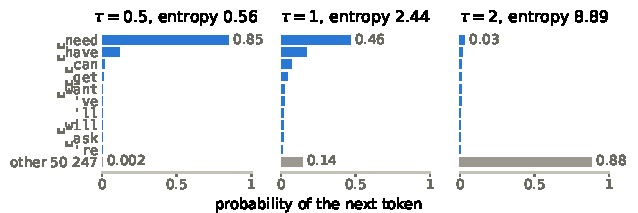
\includegraphics{sampling_temperature.pdf}

\begin{lstlisting}[style=output]
> The best way to learn mathematics is
tau=0    to learn it from a teacher.\n\nThe best way to learn mathematics is...
tau=0.7  through a teacher. You will learn how to teach, and you will learn...
tau=1.5  Hearwearill captures how in flash the Tickler microsee can portray...
\end{lstlisting}
\end{frame}


% =========================================================================
% The left column: Vaswani et al. (2017), sections 3 and 5 and table 3.  The right column: the
% papers and the configuration files of Llama 3, Qwen3, DeepSeek-V3 and V4, Kimi K2 and K3.
% Kimi K3 (July 2026), 2.78e12 parameters, is the largest model with published weights.
\begin{frame}{Since 2017: what changed, and what did not}
\footnotesize
\renewcommand{\arraystretch}{1.3}
\begin{tabularx}{\textwidth}{@{}l >{\raggedright\arraybackslash}p{0.29\textwidth} >{\raggedright\arraybackslash}X@{}}
\toprule
 & \textbf{2017} \citep{vaswani2017} & \textbf{Open models, 2024 to 2026} \\
\midrule
stack & encoder and decoder & decoder only \citep{radford2018} \\
normalization & after each sublayer & before it \citep{radford2019}; RMSNorm \citep{zhang2019} \\
positions & sinusoids added to $x_t$ & rotations of $q_t$ and $k_s$ \citep{su2024} \\
MLP & ReLU & SwiGLU \citep{shazeer2020}; each token goes to a few of many MLPs \\
attention & every head its own $K$, $V$ & heads share $K$ and $V$ \citep{ainslie2023}; compressed for long texts \citep{deepseek2026} \\
context $n$ & sentences; $512$ in GPT, 2018 & $10^5$ to $10^6$ tokens \\
parameters & $65$ million & up to $2.8\cdot10^{12}$ \citep{kimi2026} \\
\bottomrule
\end{tabularx}

\medskip
\small
\alert{Unchanged:} tokens, the scaled dot product, the sum $x+f(x)$, the next-token loss.
\end{frame}
% =========================================================================
% Part 3.  Figure: figures/part3_particles.py (particles_circle.pdf).  n = 32 tokens on the circle,
% Q = K = I, V = hI with h = 0.1, beta = 16, 20 000 layers, seed 3.  The script prints the numbers:
% 3 clusters from layer 99, 2 from layer 290, 1 from layer 14 017.  The equation is (2.3) of
% geshkovski2025 (their (SA) when Q = K = V = I); beta stands for the 1/sqrt(d) of the lecture.
\begin{frame}{Depth as time: tokens are interacting particles}
\small
A block adds to $x$: an Euler step of size $h$ \citep{lu2020}. With the normalization, which keeps $x_t$ on the sphere, layer $k$ is the time $\tau=kh$ of
\[
\frac{dx_t}{d\tau}=P^\perp_{x_t}\Big(\sum_{s=1}^n a_{ts}(x)\,Vx_s\Big),\qquad P^\perp_xy=y-\langle x,y\rangle x .
\]
\begin{center}
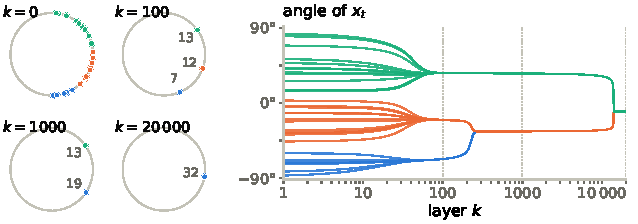
\includegraphics{particles_circle.pdf}
\end{center}
\vspace{-1.5ex}
\footnotesize
$n=32$ tokens, $d=2$, $Q=K=V=I$, $h=0.1$, and $\beta=16$ in place of $1/\sqrt d$ in $a_{ts}$.\\
\alert{The tokens cluster}: three groups at layer 100, two for thousands of layers, then one \citep{geshkovski2025}.
\end{frame}


% #########################################################################
% PART 4: TRAINING
% #########################################################################

% Part 4: training.  Figures and numbers: figures/part4_scratch.py, figures/part4_fau_corpus.py
% and figures/part4_finetune.py.

% =========================================================================
\section{Training}

% The probabilities under the tokens are those of GPT-2 small for this sentence (figures/gpt2.py);
% minus the mean of their logarithms is 4.71.
\begin{frame}[fragile]{Self-supervised learning: the text is its own label}
\centering
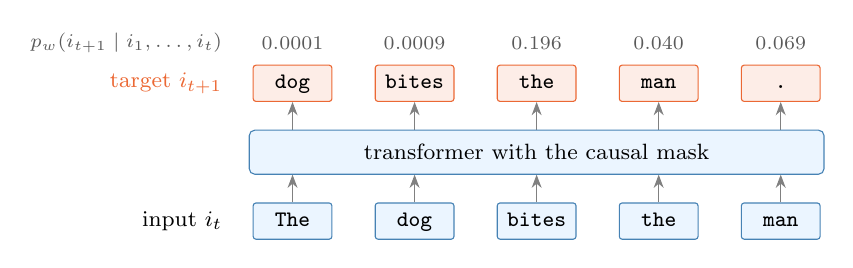
\begin{tikzpicture}[x=1.55cm, y=1mm, >=Stealth, font=\footnotesize,
    tok/.style={draw=boxframe, fill=boxbg, rounded corners=1pt, minimum height=4.6mm, minimum width=10mm,
                inner sep=1pt, font=\ttfamily\footnotesize},
    goal/.style={tok, draw=ctrl, fill=ctrl!12}]
  \foreach \t/\w/\y/\p in {0/The/dog/0.0001, 1/dog/bites/0.0009, 2/bites/the/0.196, 3/the/man/0.040, 4/man/./0.069} {
    \node[tok] (in\t) at (\t,0) {\strut\w};
    \node[goal] (out\t) at (\t,17.5) {\strut\y};
    \draw[->, black!50] (in\t.north) -- (\t,5.9);
    \draw[->, black!50] (\t,11.6) -- (out\t.south);
    \node[font=\scriptsize, text=black!65] at (\t,22.6) {$\p$};
  }
  \node[draw=boxframe, fill=boxbg, rounded corners=2pt, minimum width=7.3cm, minimum height=5.6mm] at (2,8.75)
    {transformer with the causal mask};
  \node[anchor=east, inner sep=1pt] at (-0.55,0) {input $i_t$};
  \node[anchor=east, inner sep=1pt] at (-0.55,17.5) {\ctrl{target $i_{t+1}$}};
  \node[anchor=east, inner sep=1pt, font=\scriptsize, text=black!65] at (-0.55,22.6) {$p_w(i_{t+1}\mid i_1,\dots,i_t)$};
\end{tikzpicture}

\small
\[
J(w)=-\frac1n\sum_{t=1}^{n}\log p_w\big(\ctrl{i_{t+1}}\mid i_1,\dots,i_t\big)
\]
\raggedright
The cross-entropy of lecture 04 with $|\Vocab|$ classes, and \alert{$n$ examples in one pass}: the mask hides the answers.
\begin{lstlisting}[belowskip=2pt]
i = torch.tensor([gpt2.encode("The dog bites the man.")])
F.cross_entropy(model(i[:, :-1])[0], i[0, 1:])    # targets: the text, shifted
\end{lstlisting}
\begin{lstlisting}[style=output]
> 4.705    (a uniform guess: log 50257 = 10.82)
\end{lstlisting}
\end{frame}


% =========================================================================
% Figure and numbers: figures/part4_scratch.py (scratch_loss.pdf), which prints them; the run is
% kept in data/scratch/ (results.json, checkpoints.pt).  The model is gpt2.GPT(vocab=65,
% context=128, d=128, layers=4, heads=4), initialized as GPT-2, one token per character; the text
% is tinyshakespeare.txt (1 115 394 characters, 65 distinct), the first 90% (1 003 854) for
% training, the last 10% (the end of The Taming of the Shrew, The Tempest) for validation.  2500
% steps of 16 windows of 128 characters (5 120 000 tokens, 5.1 passes over the training text),
% AdamW with eta = 1e-3 and PyTorch's other defaults, no schedule; 18.2 minutes of steps on 3
% threads of a shared CPU (22 minutes with the samples and the monitoring).  Losses at the end:
% 1.703 on the whole validation text, 1.518 on the training text; within 0.045 of each other up to
% step 500 (one pass), then the gap grows to 0.185.  Reference levels on the validation text: log 65 = 4.17, the
% character frequencies 3.35, a bigram (add-one counts of the training text) 2.48; the validation
% loss passes them between steps 15 and 20 and between 200 and 300.  The samples: prompt a newline
% (not shown), temperature 1, the generator of seed 0 at every step (the same random numbers, so
% only the weights change), the first two lines of each, cut at 70 characters (" ..." marks a cut).
\begin{frame}[fragile]{Training from scratch: one megabyte of Shakespeare}
\centering
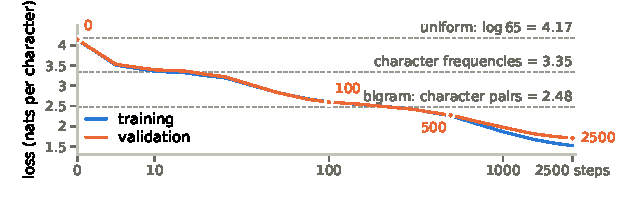
\includegraphics{scratch_loss.pdf}

\begin{lstlisting}[style=output]
step 0    t3ZrjmhPkqkARxLsXltUWRoHcu
          -eThjyU&oNdkIgAlsvSBUM ...
step 100  th remhis keswhselteelouca meaman youd Igelst, gMecofuesy h fnthek ...
          We atho y wr w keee anc
step 500  thoremhis kess selle, ouce merakn youd Ig
          Therend cofue yond nt beare hath thig berelisse. ...
step 2500 thy formed have not Warwick exckingly.
          I the regrect upon his travere hath good be else ...
\end{lstlisting}
\raggedright\footnotesize
The GPT of the slides: $818\,048$ parameters, a token per character, 18 min on a CPU.\\
\alert{First the letters, then the layout of a play, then words.}
\end{frame}


% =========================================================================
% GPT-2 small fine-tuned on public pages of FAU, on a CPU.
% Corpus: figures/part4_fau_corpus.py (crawl and cleaning; data/fau/corpus/, not in the
% repository).  Experiments and figures: figures/part4_finetune.py --train; every number below is
% in data/fau/results.json and printed by the script (without --train it only redraws).
% The corpus is what FAU serves to a program: most FAU sites (www.fau.eu, the faculties, the
% study-programme sites) answer automated requests with a proof-of-work page and were left out,
% so there are no module handbooks or examination regulations in it (see images/SOURCES.md).

% =========================================================================
% Figure: finetune_loss.pdf.  Corpus: 444 English documents for training (432 007 tokens), 19
% held out (11 620 tokens); by host: Pattern Recognition Lab 208, Department of Mathematics 87,
% FAU MoD 71, Chair of Computer Science 4 (systems) 71, others 26.  Validation: 32 fixed windows of
% 128 tokens spread over the held-out documents, every 25 steps; thin lines: the training loss of
% every step.  Both runs see the same batches in the same order.  Rates: 1e-4 from GPT-2 (the largest
% of the range considered, 3e-5 to 1e-4; no other rate tried), 6e-4 from random weights (the rate of
% GPT-3 Small, 125M parameters, Brown et al. 2020, Table 2.1, there with batches of 0.5M tokens).
% 16.5 minutes: the time of the 200 steps, on 8 threads of a shared 16-core machine.
% Validation loss from GPT-2: 3.75 -> 2.86; from random weights: 10.98 -> 6.65 (log 50257 = 10.82).
% On all the held-out text after 200 steps: 3.05 and 6.78 nats per token (perplexity 21 and 881).
\begin{frame}{Fine-tuning GPT-2 on public pages of FAU}
\small
\alert{Data}: 463 public English web pages and PDFs of FAU (mathematics, pattern recognition, systems), cleaned: $432\,007$ tokens for training, 19 pages held out.

\alert{The loop of lectures 03--04}: $J(w)$, AdamW, $B=8$ windows of $n=128$ tokens, $\eta=10^{-4}$, $200$ steps: $16$ minutes on 8 CPU threads.

\centering
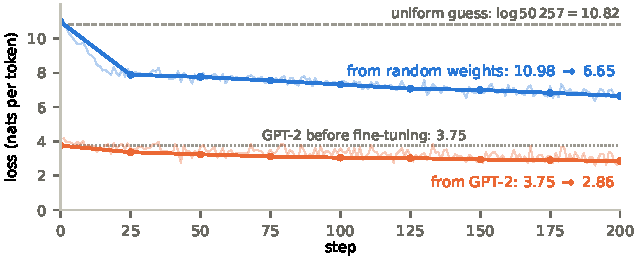
\includegraphics{finetune_loss.pdf}

\raggedright
The same loop from random weights: \alert{pretraining is the initialization}.
\end{frame}


% =========================================================================
% E4 (figures/part4_finetune.py).  Sampling: temperature 0.8, the 40 most likely tokens, 40 new
% tokens, torch.Generator seed 2 for both models; the samples are cut at the end only (...).
% All 8 prompts x 3 seeds are printed by the script and listed in images/SOURCES.md; samples that
% name real people were not chosen.  fau_probe.pdf: the prompt "FAU is a university in", the first
% of six probes (all in SOURCES).  " Erlangen" is three tokens, " Er" + "lang" + "en"; p(" Erlangen")
% is the product of their probabilities (the chain rule).  Before: 3.4e-7, after: 0.038;
% " Germany": 0.0054 -> 0.24.  E5: the longest run of tokens of a sample that also occurs verbatim
% in the training text: median 4 (GPT-2) and 6 (fine-tuned) tokens over the 24 samples, at most 20:
% the full name of the university.
\begin{frame}{Before and after fine-tuning}
\footnotesize
\renewcommand{\arraystretch}{1.05}
Sampled with $\tau=0.8$ from the 40 most likely tokens, with the same seed:

\smallskip
{\scriptsize
\begin{tabularx}{\textwidth}{@{}>{\raggedright\arraybackslash}X@{\hspace{5mm}}>{\raggedright\arraybackslash}X@{}}
\toprule
\textbf{GPT-2} & \textbf{fine-tuned} \\
\midrule
\textit{The lecture covers} many topics including history, politics and how the U.S.\ was founded, but they were all pretty long.~\dots
& \textit{The lecture covers} many topics including: - How to estimate the slope of a given slope matrix (RMS) - Representation theory and control theory~\dots \\
\bottomrule
\end{tabularx}\par}

\smallskip
The next token after \textit{FAU is a university in}:

{\centering
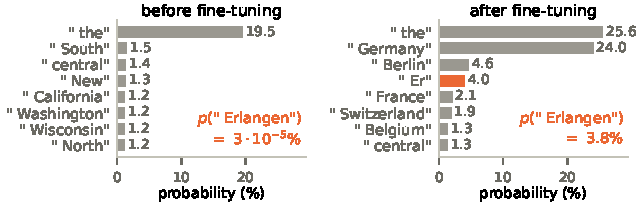
\includegraphics{fau_probe.pdf}\par}

Longest run copied from the training text: 20 tokens, the name of the university.
\end{frame}


% #########################################################################
% PART 5: AFTER PRETRAINING
% #########################################################################

% Part 5: after pretraining.  Figures and numbers: figures/part5_verifier.py; the Lean files
% are in figures/lean/.

% =========================================================================
\section{After pretraining}

% The numbers of rows 2 and 3 are those of InstructGPT (Ouyang et al., 2022, table 6): 12 725
% prompts with demonstrations; 33 207 prompts with 4 to 9 ranked answers each.  Row 1: GPT-3 was
% trained on 3e11 tokens (Brown et al., 2020), DeepSeek-V4-Pro on 3.3e13 (2026).
\begin{frame}{From completing text to solving problems}
\small
One network, one set of parameters $w$, four training signals:

\medskip
\footnotesize
\renewcommand{\arraystretch}{1.35}
\begin{tabularx}{\textwidth}{@{}l >{\raggedright\arraybackslash}X >{\raggedright\arraybackslash}p{0.27\textwidth}@{}}
\toprule
 & \textbf{Data} & \textbf{Signal} \\
\midrule
\alert{1. Pretraining} & text: $10^{11}$ to $10^{13}$ tokens \citep{brown2020,deepseek2026} & the next token \\
\alert{2. Fine-tuning} & $13\,000$ questions with answers written by people & the next token \\
\alert{3. Human feedback} & $33\,000$ questions, each with 4 to 9 answers ranked by people & a reward, fitted to the rankings \\
\ctrl{4. Verifiable reward} & problems whose answers a program can check & \ctrl{a reward, computed} \\
\bottomrule
\end{tabularx}

\medskip
\small
After steps 2 and 3, a model with $1.3\cdot10^9$ parameters was preferred to GPT-3, with $1.75\cdot10^{11}$.\footnotemark\ Steps 3 and 4 are \alert{reinforcement learning}: the model writes, and is rewarded for what it wrote.
\footnotetext{InstructGPT \citep{ouyang2022}; the numbers of rows 2 and 3 are its own.}
\end{frame}



% The identity is the policy gradient of Williams (1992); the three rows: AlphaCode filters its
% samples with the example tests; DeepSeek-R1 is rewarded for a correct final answer and, for
% code, by a compiler with test cases; AlphaProof acts in Lean and is rewarded for a checked proof.
\begin{frame}{Reinforcement learning with a verifier}
\centering
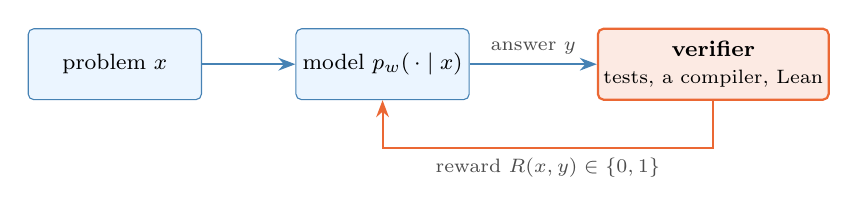
\begin{tikzpicture}[x=1mm, y=1mm, >=Stealth, font=\footnotesize,
    op/.style={draw=boxframe, fill=boxbg, rounded corners=2pt, minimum height=9mm, minimum width=22mm, inner sep=2pt, align=center},
    hot/.style={draw=ctrl, fill=ctrl!14, line width=0.8pt},
    wire/.style={->, boxframe, line width=0.7pt}]
  \node[op] (task) at (0,0) {problem $x$};
  \node[op] (model) at (34,0) {model $p_w(\,\cdot\mid x)$};
  \node[op, hot] (check) at (76,0) {\textbf{verifier}\\ {\scriptsize tests, a compiler, Lean}};
  \draw[wire] (task) -- (model);
  \draw[wire] (model) -- node[above, text=black!70, font=\scriptsize] {answer $y$} (check);
  \draw[wire, ctrl] (check.south) -- ++(0,-6) -| node[pos=0.25, below, text=black!70, font=\scriptsize] {reward $R(x,y)\in\{0,1\}$} (model.south);
\end{tikzpicture}

\small
\[
\nabla_w\,\E_{y\sim p_w(\cdot\mid x)}\big[R(x,y)\big]\;=\;\E_{y\sim p_w(\cdot\mid x)}\big[R(x,y)\,\ctrl{\nabla_w\log p_w(y\mid x)}\big]\qquad\text{\citep{williams1992}}
\]

\footnotesize
{\centering
\renewcommand{\arraystretch}{1.15}
\begin{tabular}{@{}l l l@{}}
\toprule
\textbf{The answer is} & \textbf{The verifier is} & \\
\midrule
a program & a compiler and unit tests & AlphaCode, 2022 \citep{li2022} \\
a number & a comparison with the known result & DeepSeek-R1, 2025 \citep{guo2025} \\
a proof & the kernel of Lean & AlphaProof, 2024 \citep{hubert2026} \\
\bottomrule
\end{tabular}\par}

\medskip
\small
\raggedright
No labelled answer is needed, only a check. And the loop is \alert{closed}: in pretraining the model never saw the consequences of its own text.
\end{frame}


% =========================================================================
% The figure: figures/part5_verifier.py (images/verifier_rl.pdf); the setup is in its
% docstring, and every number below is printed by it (means over the seeds 0, 1, 2).  The
% curves are p_w(correct answer | prompt), i.e. the accuracy of an answer sampled at temperature
% 1, computed exactly, on the 7290 training pairs; the 810 held-out pairs, never seen, give the
% same curves to within a point.  The curves are measured on 810 training pairs; the numbers in
% the text on all 7290 training and all 810 held-out pairs ("Mean (min - max) over seeds" in the
% output): carry pairs 25.8% -> 90.0% (T = 1), greedy 3.5% -> 99.5%; held-out carry 25.9% ->
% 89.2%, greedy 4.4% -> 99.1%; 200 more pretraining steps: 24.9%; RL from a random
% initialization: 0.13%.  Not on the slide: at the first logged RL step (10) the no-carry
% curve dips from 94.1% to 88.7% (seed 1: 83.3%) and recovers to 96.3% by step 200.
\begin{frame}{In miniature: a verifier as the reward}
\footnotesize
A transformer ($L=2$, $d=64$) pretrained on sums in which 70\% of the carries are forgotten (\texttt{37+58=85.}), then rewarded: $R=1$ if Python finds the answer right, else $0$.
\[
\nabla_w J=\E\big[(R-b)\,\nabla_w\log p_w(y\mid x)\big],\qquad b=\text{mean reward of 8 answers $y$ to $x$}.
\]
\centering
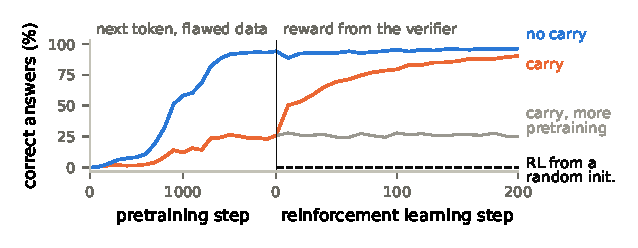
\includegraphics{verifier_rl.pdf}

\raggedright
Sums with a carry: $26\%\to90\%$ right (greedy: $3.5\%\to99.5\%$); on 810 held-out sums, $26\%\to89\%$.

\alert{Pretraining imitates the data, mistakes included; the verifier rewards correctness}, with no correct answer ever shown.
\end{frame}


% =========================================================================
% The two Lean files are figures/lean/sum_odd.lean and figures/lean/sum_odd_wrong.lean, shown
% whole (so the line numbers of the error, 11:37 and 9:14, are the numbers in the margin),
% checked with Lean 4.35.0, core library, no Mathlib: `lean sum_odd.lean`.  The outputs are
% copied from that command; the error is shortened by cutting lines only (the omega
% counterexample "a possible counterexample may satisfy the constraints ..." and the hypotheses
% of the goal).  Lean prints the goal after the Unicode turnstile; it is typeset as $\vdash$
% (mathescape), since pdflatex and listings take only ASCII.
% The wrong step forgets the +1 of (k+1)^2 = k^2 + 2k + 1, as the model of the next slide
% forgets the carry.  Trusted when Lean accepts: its small kernel [de Moura and Ullrich 2021,
% Sec. 5]; not checked: that the statement says what we mean.
\begin{frame}[fragile,t]{A proof checker does not trust the model}
\footnotesize
\lstset{aboveskip=2pt, belowskip=2pt, numbers=left, numberstyle=\tiny\color{gray}, numbersep=7pt}
$1+3+\dots+(2n-1)=n^2$, by induction on $n$, in Lean\footnotemark:
\begin{onlyenv}<1>
\begin{lstlisting}[style=lean]
-- checked with Lean 4.35.0 (core library, no Mathlib)
def sumOdd : Nat -> Nat               -- 1 + 3 + ... + (2n - 1)
  | 0     => 0
  | n + 1 => sumOdd n + (2 * n + 1)

theorem sumOdd_eq (n : Nat) : sumOdd n = n * n := by
  induction n with
  | zero => rfl
  | succ k ih => rw [sumOdd, ih, Nat.add_mul, Nat.mul_add]; omega

#print axioms sumOdd_eq
\end{lstlisting}
\begin{lstlisting}[style=output, numbers=none]
> 'sumOdd_eq' depends on axioms: [propext, Quot.sound]
\end{lstlisting}
\alert{Accepted}: every step is checked by Lean's small kernel. Not checked: that the statement says what we mean.
\end{onlyenv}
\begin{onlyenv}<2>
\begin{lstlisting}[style=lean]
-- checked with Lean 4.35.0 (core library, no Mathlib)
def sumOdd : Nat -> Nat               -- 1 + 3 + ... + (2n - 1)
  | 0     => 0
  | n + 1 => sumOdd n + (2 * n + 1)

theorem sumOdd_eq (n : Nat) : sumOdd n = n * n := by
  induction n with
  | zero => rfl
  | succ k ih =>
    have step : (k + 1) * (k + 1) = k * k + 2 * k := by
      rw [Nat.add_mul, Nat.mul_add]; omega
    rw [sumOdd, ih, step]
\end{lstlisting}
\begin{lstlisting}[style=error, numbers=none, mathescape]
> sum_odd_wrong.lean:11:37: error: omega could not prove the goal:
> sum_odd_wrong.lean:9:14: error: unsolved goals
> $\vdash$ k * k + (2 * k + 1) = k * k + 2 * k
\end{lstlisting}
\alert{Rejected}, at the false step: $(k+1)^2=k^2+2k$ forgets the $+1$.
\end{onlyenv}
\footnotetext{Lean 4 \citep{demoura2021}. \texttt{omega}: a decision procedure for linear arithmetic.}
\end{frame}


% =========================================================================
% Sources, each read on its primary page: AlphaProof (Hubert et al., Nature 2026, and the DeepMind
% post of 25 July 2024: problems 1, 2 and 6, problem 4 by AlphaGeometry 2, graded 28/42; the reward
% is -1 per tactic); Gemini Deep Think (DeepMind, 21 July 2025: 35/42, natural language, graded by
% the coordinators of the Olympiad); Aristotle (Harmonic, arXiv:2510.01346: five problems in Lean);
% AxiomProver (github.com/AxiomMath/IMO2026: six problems, statements and proofs generated, checked
% by Lean, not graded by the Olympiad); Fermat's Last Theorem (Anthropic, 4 September 2026: 13
% million lines of Lean in 11 days, following a known proof); the quote: T. Hales, 9 October 2026.
\begin{frame}{Lean as the judge, 2024 to 2026}
\footnotesize
\renewcommand{\arraystretch}{1.25}
\begin{tabularx}{\textwidth}{@{}l >{\raggedright\arraybackslash}X@{}}
\toprule
\alert{July 2024} & AlphaProof: reinforcement learning in Lean, reward $-1$ per step of the proof. With AlphaGeometry, 4 of the 6 problems of the Mathematical Olympiad: 28 of 42 points \citep{hubert2026}. \\
\alert{July 2025} & Gemini Deep Think: 5 problems, 35 points, a gold medal; in natural language, graded by the Olympiad's coordinators \citep{luong2025}. Aristotle: 5 problems, in Lean \citep{achim2025}. \\
\alert{July 2026} & AxiomProver: all 6 problems in Lean, statements included; checked by Lean, not graded by the Olympiad \citep{axiom2026}. \\
\alert{Sept.\ 2026} & Fermat's Last Theorem in Lean: 13 million lines written by a language model in 11 days, along a known proof \citep{anthropic2026b}. \\
\bottomrule
\end{tabularx}

\medskip
\begin{mathbox}{T.~Hales, October 2026 \citep{hales2026}}
``Lean proofs should never be believed until they have been checked by the kernel. Additionally, a proof in Lean should not be accepted until a human audit is performed to ensure statement fidelity.''
\end{mathbox}
\end{frame}


% =========================================================================
% Every number is one of a slide above: tokens per word (part 1), the recall task (part 2), the
% parameter counts (part 3), the two training runs (part 4), the miniature of part 5.
\begin{frame}{Key takeaways}
\footnotesize
\begin{enumerate}
\item \alert{Tokens.} The model reads integers. GPT-2 cuts text into $50\,257$ pieces, learned by merging frequent pairs of bytes: $1.15$ tokens per English word, $2.82$ per German word.
\item \alert{Attention.} A differentiable look-up table, $\sum_s\softmax_s(\langle q,k_s\rangle)\,v_s$. The score is from 2015; in 2017 the recurrent network was removed: any two tokens are one step apart.
\item \alert{Symmetry.} Self-attention is permutation equivariant. The order of the text enters through the positions and the mask only.
\item \alert{Transformer.} $x\leftarrow x+\Attention(\LN(x))$, $x\leftarrow x+\MLP(\LN(x))$, $L$ times: 32 lines of code and, for GPT-2, $124\,439\,808$ parameters, $45.5\%$ of them in the MLPs. Depth is time: the tokens are interacting particles, and they cluster.
\item \alert{Training.} The text is its own label: $n$ examples in one pass. From random weights on Shakespeare, $4.14\to1.70$ nats per character. Pretraining is the initialization: on pages of FAU, $3.75\to2.86$ nats per token in 200 steps from GPT-2, $10.98\to6.65$ from random weights.
\item \alert{After pretraining.} Reinforcement learning closes the loop: the model is rewarded for what it writes. Where a program checks the answer (tests, a compiler, Lean), no labels are needed: $26\%\to90\%$ in our miniature.
\end{enumerate}
\end{frame}


% #########################################################################
% APPENDIX
% #########################################################################

% Not part of the lecture: the vision transformer, and the details behind some frames of parts 2
% and 3, kept for questions.  Its section page has neither a number nor the diagram, and \appendix
% keeps it out of the outline.
\appendix
\setbeamertemplate{section page}{%
  \centering
  {\usebeamercolor[fg]{section title}\usebeamerfont{section title}\LARGE\insertsectionhead\par}}
\section{Appendix}

% #########################################################################
% APPENDIX: VISION TRANSFORMERS
% #########################################################################
% Figures and numbers: figures/appendix_vit.py.  The statements and numbers of the paper:
% Dosovitskiy et al. (2021), arXiv:2010.11929v2 (the ICLR version), at the places named above
% each frame.

% =========================================================================
% The digit and the sequence: figures/appendix_vit.py (vit_digit.pdf, vit_sequence.pdf; test
% digit 1 of MNIST, a 2, cut into 16 patches of 7 x 7 pixels).  The model: Eq. (1)-(4) of the
% paper; "the grid enters only through the cut": Section 3.1, "Inductive bias" (the other entry
% point, interpolating p_t when the resolution changes, is not used here).  ViT-B/16: Table 1
% (12 layers, D = 768, MLP 3072, 12 heads, 86M parameters) and Appendix B.1 (resolution 224,
% so 224^2 / 16^2 = 196 patches).
\begin{frame}{Vision transformers: an image is a sequence of patches}
\small
\begin{columns}[c]
\begin{column}{0.33\textwidth}
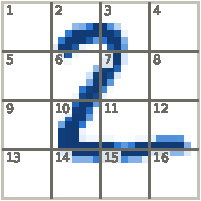
\includegraphics{vit_digit.pdf}
\end{column}
\begin{column}{0.65\textwidth}
$16$ patches $\pi_t\in\R^{49}$ of $7\times7$ pixels, row by row:
\[
x_t=E\,\pi_t+\ctrl{p_t},\qquad x_0=\ctrl{x_{\mathrm{cls}}}+\ctrl{p_0},
\]
$E\in\R^{d\times49}$, all learned. Then $L$ blocks of part~3 \alert{without the mask}; the class is read from $x_0$.
\end{column}
\end{columns}

\medskip
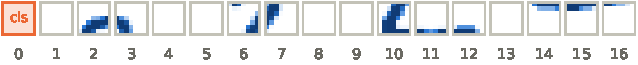
\includegraphics{vit_sequence.pdf}

\medskip
\footnotesize
\alert{No convolution:} the grid enters only through the cut into patches \citep{dosovitskiy2021}.\\
ViT-B/16: $196$ patches of $16\times16$ pixels, $L=12$, $d=768$, $H=12$; $86$M parameters.
\end{frame}


% =========================================================================
% The listing is the class ViT of figures/appendix_vit.py, line for line; Block is the block of
% part 3 (gpt2.Block) without its two lines of mask.  Every network trained with the loop of
% lecture 02: cross-entropy, Adam with learning rate 1e-3, batches of 64, 4690 steps (5 epochs),
% seeds 0 (weights) and 1 (shuffling).  The script trains the two networks of lecture 04 again
% (figures/part2_mnist.py there) and reproduces their errors.
\begin{frame}[fragile]{A vision transformer on the digits}
\begin{lstlisting}
class ViT(nn.Module):
    def __init__(self, d=64, L=4, H=4):
        super().__init__()
        self.E = nn.Linear(49, d)                          # a 7x7 patch -> R^d
        self.cls = nn.Parameter(torch.zeros(1, 1, d))      # the class token
        self.p = nn.Parameter(0.02 * torch.randn(17, d))   # p_0, ..., p_16
        self.blocks = nn.Sequential(*[Block(d, H) for _ in range(L)])
        self.out = nn.Sequential(nn.LayerNorm(d), nn.Linear(d, 10))

    def forward(self, img):                                # img: (B, 784)
        x = img.view(-1, 28, 28).unfold(1, 7, 7).unfold(2, 7, 7)
        x = self.E(x.reshape(-1, 16, 49))                  # 16 patches -> R^d
        x = torch.cat([self.cls.expand(len(x), -1, -1), x], 1) + self.p
        return self.out(self.blocks(x)[:, 0])              # read out x_0
\end{lstlisting}
\footnotesize
\begin{columns}[c]
\begin{column}{0.36\textwidth}
\raggedright
\texttt{Block}: part~3, without the mask. All three trained by the loop of lecture~02: Adam, 5~epochs.
\end{column}
\begin{column}{0.62\textwidth}
\renewcommand{\arraystretch}{1.05}
\begin{tabular}{@{}l r r@{}}
\toprule
 & parameters & test error \\
\midrule
fully connected & $118\,282$ & $2.2\%$ \\
convolutional & $5\,994$ & $1.3\%$ \\
\alert{vision transformer} & $205\,066$ & $2.4\%$ \\
\bottomrule
\end{tabular}
\end{column}
\end{columns}
\end{frame}


% =========================================================================
% figures/appendix_vit.py (vit_data.pdf): each network trained for 4690 steps (5 epochs of the
% 60 000 digits) on the first N training digits, one run per point, test error on the 10 000
% test digits after the last step.  Test errors (%), N = 1000, 4000, 16000, 60000:
% fully connected 12.36, 6.96, 3.65, 2.24; CNN 5.84, 2.46, 1.48, 1.28; ViT 17.23, 5.86, 4.06,
% 2.37.  Ratio ViT/CNN: 3.0, 2.4, 2.7, 1.9 (not monotone: one run per point, and at N = 16000
% the ViT still has 1.31% training error).  In this budget the ViT is no better than the fully
% connected network: it is still learning (training error 1.76% at N = 60000).
% The paper: Section 4.3 and Figure 3 ("The BiT CNNs outperform ViT on ImageNet, but with the
% larger datasets, ViT overtakes"); Table 5 (ViT-B/16 pre-trained on ImageNet, then fine-tuned
% on ImageNet at resolution 384: 77.91%); Table 2 (pre-trained on JFT-300M: ViT-H/14
% 88.55 +- 0.04%, BiT-L = ResNet152x4 87.54 +- 0.02%); dataset sizes: Section 4.1.
\begin{frame}{Built-in symmetry saves data}
\begin{columns}[c]
\begin{column}{0.52\textwidth}
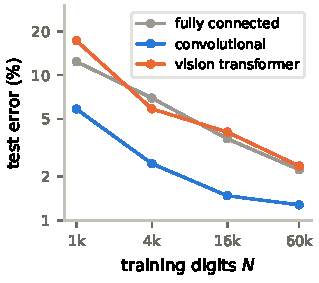
\includegraphics{vit_data.pdf}
\end{column}
\begin{column}{0.46\textwidth}
\footnotesize
4690 steps of Adam on the first $N$ digits.

\medskip
\alert{The CNN with $4\,000$ digits} ($2.46\%$) is about as good as the transformer with $60\,000$ ($2.37\%$).

\medskip
The transformer's error: $3.0$ times the CNN's at $N=1\,000$, $1.9$ times at $60\,000$.

\medskip
\begin{mathbox}{ImageNet, top-1 \citep{dosovitskiy2021}}
Pre-trained on ImageNet ($1.3$M images): ViT-B/16 $77.91\%$, below the ResNets.\\[2pt]
On JFT-300M ($303$M images): ViT-H/14 \alert{$88.55\%$}, the ResNet BiT-L $87.54\%$.
\end{mathbox}
\end{column}
\end{columns}
\end{frame}


% =========================================================================
% OPTIONAL.  figures/appendix_vit.py (vit_attention.pdf): the ViT of the previous slides
% (60 000 digits).  The weights a_0s of the class token over the 16 patches, averaged over the
% 4 heads, in blocks 1 and 4, for test digits 1, 2, 3, 4 and 7; the orange of a patch is its
% weight relative to the largest.  The numbers below: over the first 1000 test digits.
% (The similarity of the learned positions, Figure 7 of the paper, is not shown: on this
% model it has no visible grid structure; see vit_positions.pdf and the printed numbers.)
\begin{frame}{Where the class token looks}
\centering
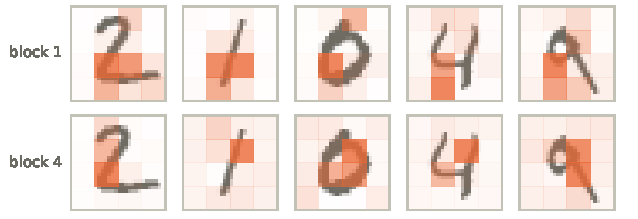
\includegraphics{vit_attention.pdf}

\medskip
\raggedright
\small
$a_{0s}(x)$: the weight of patch $s$ for the class token, averaged over the $4$ heads.

\medskip
Over $1\,000$ test digits, the largest weight on one patch is $0.30$ in block~1 and $0.34$ in block~4 on average; equal weights would give $1/17\approx0.06$.
\end{frame}


% =========================================================================
% E1 and the end of E2 (figures/part4_finetune.py).  J: mean -log p_w of the next token over
% non-overlapping windows of 128 tokens (at most 160 windows, evenly spread, per text: FAU English
% 11 520 tokens, the others 18 048-20 480).  FAU: the held-out documents, never trained on.
% Wikipedia: the articles Photosynthesis, Bicycle, Volcano, Chess, Coffee (plain text from the
% API, revision ids in results.json).  Shakespeare: the first 60 000 characters of
% notebooks/data/tinyshakespeare.txt.  GPT-2's training text WebText had all Wikipedia documents
% removed (Radford et al. 2019, Sec. 2.1) and non-English pages too (Sec. 3.7).
% Per word: J times tokens per word (words: separated by white space), so that texts with
% different tokenizations compare; German/English FAU: x1.72 tokens per word, x1.94 per word.
% Perplexity e^J of the FAU text: 47.6 before, 21.1 after; Wikipedia 36.1 -> 46.1.
\begin{frame}{Fine-tuning in detail: the loss on held-out text}
\small
\centering
\renewcommand{\arraystretch}{1.12}
\begin{tabular}{@{}l r r r r@{}}
\toprule
 & tokens & \multicolumn{2}{c}{GPT-2} & fine-tuned \\
\cmidrule(lr){3-4}\cmidrule(l){5-5}
held-out text & per word & $J$ & per word & $J$ \\
\midrule
FAU, English (19 documents) & $1.72$ & $3.86$ & $6.66$ & \alert{$3.05$} \\
Wikipedia (5 articles) & $1.34$ & $3.59$ & $4.82$ & $3.83$ \\
Shakespeare & $1.68$ & $4.83$ & $8.13$ & \\
FAU, German (17 documents) & $2.97$ & $4.36$ & $12.95$ & $4.36$ \\
\bottomrule
\end{tabular}\par

\medskip
\raggedright
$J$ in nats per token; per word: $J$ times tokens per word.

\medskip
GPT-2 was trained on English web pages.\footnotemark{} German costs $1.7$ times the tokens per word and $1.9$ times the nats per word.

\medskip
\alert{Fine-tuning}: FAU text $-0.81$, Wikipedia $+0.24$ nats per token.
\footnotetext{Without Wikipedia and without non-English pages \citep{radford2019}.}
\end{frame}


% =========================================================================
% Appendix.  Statements checked against arXiv:2312.10794v5 (= Bull. AMS 62 (2025) 427-479):
% Lemma 6.4 (cone collapse; any n >= 1, d >= 2, beta > 0, V = I, any fixed Q, K) and Theorem 6.1
% (due to Markdahl et al. 2018 and Criscitiello et al. 2026; n >= 2, d >= 3, beta >= 0, Q = K = V = I).
% Mean field: their (3.1)-(3.4); the energy: (3.5)-(3.6) and Proposition 3.4.  Metastability:
% geshkovski2024, Theorem 1.2 (d, n >= 2, beta > 1, tokens starting in k separated caps: they stay
% there up to a time T_2 >= (eps/n) e^{(1-alpha) beta}).
\begin{frame}{Depth as time in detail: clustering}
\footnotesize
\begin{mathbox}{Theorem (\citet{geshkovski2025}, Lemma 6.4 and Theorem 6.1)}
Let $\beta>0$, $V=I$, $a_{ts}=\softmax_s(\beta\langle Qx_t,Kx_s\rangle)$, and let $x_t(\tau)\in\mathbb S^{d-1}$ solve the equation of part~3.
\begin{enumerate}
\item For any fixed $Q,K$: if all $x_t(0)$ lie in an open hemisphere, there are $x^*$ and $C,\lambda>0$ with $|x_t(\tau)-x^*|\le Ce^{-\lambda\tau}$ for all $t$ and $\tau\ge0$.
\item For $Q=K=I$ and $d\ge3$: for almost every $x(0)$ there is $x^*$ with $x_t(\tau)\to x^*$ for all $t$.
\end{enumerate}
\end{mathbox}
\begin{itemize}
\item \alert{Scope.} Constant weights, one head, no MLP, continuous time, $\tau\to\infty$: not trained weights, not finite depth. Before the limit, groups persist for a time exponential in $\beta$ \citep{geshkovski2024}; with hardmax attention, several clusters set by \emph{leaders} \citep{alcalde2025}.
\item \alert{Mean field.} $\mu_\tau=\frac1n\sum_t\delta_{x_t(\tau)}$ solves $\partial_\tau\mu+\operatorname{div}(X[\mu]\,\mu)=0$ \citep{sander2022}, with $X[\mu](x)=P^\perp_x\big(\int e^{\beta\langle x,y\rangle}y\,d\mu(y)\big/\!\int e^{\beta\langle x,y\rangle}d\mu(y)\big)$. The energy $\frac1{2\beta}\iint e^{\beta\langle x,y\rangle}d\mu\,d\mu$ increases along it; its maximizers are the Dirac masses.
\item \alert{Control.} Time is depth, the state is the $n$ tokens (or $\mu_\tau$), the \ctrl{control} is the weights $(Q,K,V)$ and MLP of each layer: one control for all prompts. Controllability becomes exact interpolation of sequences and of measures \citep{alcalde2026,geshkovski2026}.
\end{itemize}
\end{frame}


% =========================================================================
% Theorems 2 and 3 of Yun et al. (ICLR 2020), checked against arXiv:1912.10077: T^{2,1,4} is the
% class of networks with 2 heads of size 1 and a feed-forward width of 4; the distance is the L^p
% distance with the entrywise l_p norm.  Their blocks have no layer normalization and no mask.
\begin{frame}{Universal approximation with transformers}
\small
The density theorem of lecture 02, for sequences:
\begin{mathbox}{Theorem (\citet{yun2020})}
Let $1\le p<\infty$ and $\varepsilon>0$. For every continuous and permutation-equivariant $f\colon\R^{n\times d}\to\R^{n\times d}$ with compact support there is a transformer $g$, with $2$ heads of width $1$ and MLPs of width $4$, such that
\[
\Big(\int\|f(X)-g(X)\|_p^p\,dX\Big)^{1/p}\le\varepsilon .
\]
With positions $E\in\R^{n\times d}$ added to the input, $X\mapsto g(X+E)$, the same holds for every continuous $f$ on a compact set.
\end{mathbox}
\footnotesize
\begin{itemize}
\item \alert{Without positions} a transformer is permutation equivariant, and these are the only functions it reaches. \alert{With positions}, all of them.
\item The width does not depend on $n$ or $d$. The depth does: of order $n\,\delta^{-dn}$ blocks for a resolution $\delta$.
\item Their blocks: softmax attention and a ReLU MLP, without normalization and without mask.
\end{itemize}
\end{frame}


% =========================================================================
% Section 3.5 of Vaswani et al. (2017) for the sinusoids; Su et al. (2024), eq. 11-16, for the
% rotary embeddings.  The table: the model papers and the configuration files of the models.
\begin{frame}{Positions in detail: from sums to rotations}
\small
\alert{2017:} add $p_t=(\sin\omega_jt,\cos\omega_jt)_j$ to the token. Then $p_{t+k}=R_k\,p_t$ for a rotation $R_k$ that does not depend on $t$: a shift of the text is a linear map.

\medskip
\alert{Today:} rotate the query and the key themselves \citep{su2024}. In the plane $\R^2=\mathbb C$,
\[
q_t=(Qx_t)\,e^{\mathrm it\theta},\ \ k_s=(Kx_s)\,e^{\mathrm is\theta}
\quad\Longrightarrow\quad
\langle q_t,k_s\rangle=\operatorname{Re}\big[(Qx_t)\,\overline{(Kx_s)}\,e^{\mathrm i(t-s)\theta}\big],
\]
and in $\R^d$, $d/2$ planes with the angles $\theta_j=10000^{-2j/d}$. \alert{The score sees only $t-s$.}

\medskip
\footnotesize
{\centering
\renewcommand{\arraystretch}{1.1}
\begin{tabularx}{\textwidth}{@{}l >{\raggedright\arraybackslash}X@{}}
\toprule
a learned vector $p_t$ for each $t\le1024$ & GPT-2, 2019 \\
a learned number added to the score, by distance & T5, 2020 \citep{raffel2020} \\
rotations & LLaMA, 2023 \citep{touvron2023}; Llama 3, Mistral, Qwen3, DeepSeek-V3 \\
\bottomrule
\end{tabularx}\par}
\end{frame}


% =========================================================================
% Figure and numbers:
% figures/part1_embeddings.py (positions_similarity.pdf: every 4th position, t, s = 0..1020).
\begin{frame}{Positions in detail: what GPT-2 learned}
\centering
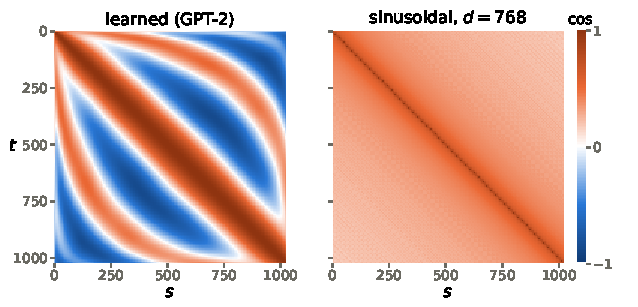
\includegraphics{positions_similarity.pdf}

\raggedright\footnotesize
$\cos(p_t,p_s)$. Sinusoidal: a function of $t-s$. Learned: on average $0.99$ for $|t-s|=8$, $0.73$ for $64$, $-0.45$ for $256$; a function of $t-s$ explains $80\%$ of its variance. Three directions carry $90\%$ of the variance of the $p_t$.
\end{frame}


% =========================================================================
\begin{frame}[allowframebreaks]{References}
\scriptsize
\bibliographystyle{plainnat}
\bibliography{self_attention_and_transformers}
\end{frame}

\end{document}
